\subsection{霍普夫空间}

定义 2. --- 霍普夫空间是一个带基点拓扑空间 (X, e)，配备连续合成法则 m: X × X → X，使得

\begin{enumerate}
\def\labelenumi{(\roman{enumi})}
\item
  \(m(e, e) = e\) ;
\item
  存在以 \(e\) 为基点的同伦，将映射 \(x \mapsto m(x, e)\) 和 \(x \mapsto m(e, x)\) 与映射 \(\mathrm{Id}_{\mathrm{X}}\) 联系起来。
\end{enumerate}

有时把性质 (i) 和 (ii) 表述为：e 是合成法则 m 的同伦意义下的单位元。

注意，在拓扑空间 X 上的连续合成法则 m 可能有多个同伦意义下的单位元。例如，当 \(X = \mathbf{R}\) 且 \(m(x, y) = (x + y)/2\) 时，每个 \(x \in \mathbf{R}\) 都是同伦意义下的单位元。

例。--- 1) 设 G 是拓扑群，m 是其合成法则。G 的单位元 e 是同伦意义下的单位元，且 (G, e) 是霍普夫空间。

\begin{enumerate}
\def\labelenumi{\arabic{enumi})}
\setcounter{enumi}{1}
\tightlist
\item
  设 X 是拓扑空间，x 是 X 中的一点。赋予带基点空间 \((\Omega_{x}(\mathrm{X}), e_{x})\) 以 x 处圈的拼接后，它是一个霍普夫空间。事实上，首先有 \(e_{x} * e_{x} = e_{x}\)。另一方面，设 \(\psi: I \to I\) 是如下定义的函数：\(\psi(t) = 2t\) 当 \(0 \leqslant t \leqslant \frac{1}{2}\) 时，并且 \(\psi(t) = 1\) 当 \(\frac{1}{2} \leqslant t \leqslant 1\) 时（参见 III, 第~291~页）；设 \(\sigma: I \times I \to I\) 是将 \(\psi\) 与 \(\mathrm{Id}_{\mathrm{I}}\) 连接起来的严格同伦（III, 第~289~页，例）。于是，对于每个圈 \(c \in \Omega_{x}(\mathrm{X})\)，映射 \(c \circ \sigma: I \times I \to X\) 是将 \(c * e_{x}\) 与 c 在 \(\Omega_{x}(\mathrm{X})\) 中连接起来的严格同伦。
\end{enumerate}

令 \(\tau\) 为映射 \(\Omega_x(\mathrm{X}) \times \mathbf{I} \to \Omega_x(\mathrm{X})\)，其定义为 \(\tau(c, s)(t) = c \circ \sigma(s, t)\)。证明 \(\tau\) 连续。根据 III, 第~257~页的命题 1，只需证明映射 \((c, s, t) \mapsto c(\sigma(s, t))\) 从 \(\Omega_x(\mathrm{X}) \times \mathbf{I} \times \mathbf{I}\) 到 X 连续；也就是说，由于 \(\mathbf{I} \times \mathbf{I}\) 紧，只需证明映射 \(c \mapsto c \circ \sigma\) 从 \(\mathcal{C}_c(\mathbf{I};\mathrm{X})\) 到 \(\mathcal{C}_c(\mathbf{I} \times \mathbf{I};\mathrm{X})\) 连续。最后一个断言由 I, 第~132~页的引理 b) 得出。因此，映射 \(\tau\) 是将映射 \(c \mapsto c * e_x\) 与 \(\Omega_x(\mathrm{X})\) 的恒等映射连接起来的同伦。映射 \(\tau(e_x, s)(t) = x\) 对所有 \(s, t \in I\) 都成立，所以 \(\tau\) 是在 \(e_x\) 处的带基点同伦。对映射 \(c \mapsto e_x * c\) 作同样论证。

命题 3. — 设 (X, e) 是霍普夫空间，m: X × X → X 是其合成法则。对于 X 中在 e 处的任意圈 c、c′，有：

\[
c ^ {\prime} * c \sim c * c ^ {\prime} \sim m \circ (c, c ^ {\prime}),
\]

其中 ∼ 表示严格同伦关系。群 \(\pi_{1}(\mathrm{X},e)\) 的群法则是以下两个映射的复合：规范同构 \(\pi_{1}(\mathrm{X},e)\times\pi_{1}(\mathrm{X},e)\to\pi_{1}(\mathrm{X}\times\mathrm{X},(e,e))\)（III, 第~297~页，推论）和同态 \(\pi_{1}(m,(e,e))\)，后者从 \(\pi_{1}(\mathrm{X}\times\mathrm{X},(e,e))\) 到 \(\pi_{1}(\mathrm{X},e)\)。群 \(\pi_{1}(\mathrm{X},e)\) 是交换的。

令 \(\mu\colon\pi_{1}(\mathrm{X},e)\times\pi_{1}(\mathrm{X},e)\to\pi_{1}(\mathrm{X},e)\) 为由规范同构 \(\pi_{1}(\mathrm{X},e)\times\pi_{1}(\mathrm{X},e)\) 到 \(\pi_{1}(\mathrm{X}\times\mathrm{X},(e,e))\) 与同态 \(\pi_{1}(m,(e,e))\) 的复合给出的群同态。还需证明：

\[
\mu (\gamma , \gamma^ {\prime}) = \gamma \gamma^ {\prime} = \gamma^ {\prime} \gamma\tag{1}
\]

对于所有 \(\gamma, \gamma' \in \pi_1(X, e)\)。根据 III, 第~297~页的注 2，有：

\[
\mu (\gamma , \gamma^ {\prime}) = \mu (\gamma , \varepsilon_ {e}) \mu (\varepsilon_ {e}, \gamma^ {\prime}) = \mu (\varepsilon_ {e}, \gamma^ {\prime}) \mu (\gamma , \varepsilon_ {e}).\tag{2}
\]

设 \(c \in \Omega_e(\mathrm{X})\) 是类为 \(\gamma\) 的圈，并将映射 \(m_1 \colon \mathrm{X} \to \mathrm{X}\) 记为由 \(m_1(x) = m(x, e)\) 定义的映射；于是，\(\mu(\gamma, \varepsilon_e)\) 是 \(m_1 \circ c\) 的类。根据霍普夫空间的定义，以 \(e\) 为基点的映射 \(m_1\) 和 \(\mathrm{Id_X}\) 在 \(e\) 处具有相同的带基点同伦类。因此，在 \(e\) 处的圈 \(m_1 \circ c\) 和 \(c\) 严格同伦（III, 第~296~页，命题 3 的推论 1），从而 \(\mu(\gamma, \varepsilon_e) = \gamma\)。同理可得 \(\mu(\varepsilon_e, \gamma') = \gamma'\)。关系式 (1) 随即由关系式 (2) 得出。

注。--- 设 \((X,e)\) 是霍普夫空间。根据命题 3，道路类的合成映射 \(\pi_{1}(X,e)\times\pi_{1}(X,e)\to\pi_{1}(X,e)\) 是连续的，只要给 \(\pi_{1}(X,e)\) 赋予由 \(\Lambda_{e}(X)\) 上的紧收敛拓扑所诱导的商拓扑。事实上，这就是连续同构 \(\pi_{1}(X,e)\times\pi_{1}(X,e)\to\pi_{1}(X\times X,(e,e))\)（III, 第~298~页，注 3）与连续映射 \(m_{*}:\pi_{1}(X\times X,(e,e))\to\pi_{1}(X,e)\)（III, 第~294~页，注 1）的复合。

\subsection{拓扑群的庞加莱群}

若 G 是拓扑群，则对每个 \(g \in G\)，左平移 \(x \mapsto gx\) 都是 G 到自身的同胚（TG, III, 第~2~页），并诱导出从 \(\pi_{1}(G, e)\) 到 \(\pi_{1}(G, g)\) 的同构。

设 G 是拓扑群，e 是其单位元，并以 \(G_{0}\) 表示 G 中 e 的道路连通分支。以 R 表示 G 上其等价类为 G 的道路连通分支的等价关系，并令 \(p: G \to \pi_{0}(G)\) 为规范映射。由于每个左平移或右平移都是 G 的同胚，关系 R 对 G 的群法则在左、右两侧都相容。根据 A, I, 第~35~页的定理 2，群 \(G_{0}\) 是 G 的正规子群，商群 \(G/G_{0}\) 等于赋予 G 所诱导的合成法则的 \(\pi_{0}(G)\)，且映射 p 是群同态。

群 \(\pi_{1}(G,e)\) 称为 G 的庞加莱群，记作 \(\pi_{1}(G)\)。从 \(G_{0}\) 到 G 的规范嵌入诱导出从 \(\pi_{1}(G_{0})\) 到 \(\pi_{1}(G)\) 的同构（III, 第~293~页，注 2）。

设 \(g\) 是 G 的一个元素；右平移 \(\boldsymbol{\delta}_g \colon x \mapsto xg\) 诱导出同构 \((\boldsymbol{\delta}_g)_* \colon \pi_1(\mathrm{G}) \to \pi_1(\mathrm{G}, g)\)。设 \(g\) 属于 \(\mathrm{G}_0\)，并令 \(b\) 为连接 \(e\) 与 \(g\) 的道路。映射 \(\sigma \colon \mathrm{G} \times \mathbf{I} \to \mathrm{G}\) 由 \(\sigma(x, t) = xb(t)\) 定义，是将 \(\mathrm{Id}_{\mathrm{G}}\) 与 \(\boldsymbol{\delta}_g\) 连接起来的同伦。根据 III, 第~295~页的命题 3，对于每个 \(\alpha \in \pi_1(\mathrm{G})\)，有 \((\boldsymbol{\delta}_g)_*(\alpha) = \beta^{-1}\alpha\beta\)，其中 \(\beta \in \varpi_{e,g}(\mathrm{G})\) 是道路 \(b\) 的类。若以 \(\gamma_g\) 表示左平移 \(x \mapsto gx\)，同样有 \((\gamma_g)_*(\alpha) = \beta^{-1}\alpha\beta\)。

对每个 \(g \in G\)，映射 \(\operatorname{Int}(g)\) : \(G \to G\) 都诱导出 \(\pi_{1}(\operatorname{Int}(g))\) 在 \(\pi_{1}(G)\) 上的一个自同构。于是定义 G 在 \(\pi_{1}(G)\) 上的作用。对于所有 \(g \in G\)，有 \(\pi_{1}(\operatorname{Int}(g)) = (\boldsymbol{\gamma}_{g^{-1}})_{*} \circ (\boldsymbol{\delta}_{g})_{*}\)，因此子群 \(G_{0}\) 的作用是平凡的；这就给出了 \(\pi_{0}(G)\) 在 \(\pi_{1}(G)\) 上的作用。当 G 是交换群时，此作用是平凡的，但并非总是如此（IV, 第~459~页，习题 1）。

\subsection{拓扑群的覆叠}

命题 4. --- 设 (X, e) 是霍普夫空间（IV, 第~373~页，定义 2），m: X × X → X 是其合成法则。假设空间 X 连通且局部道路连通。设 X' 是 X 的连通覆叠；以 p 表示其投影，并令 e' 为纤维 \(X'_{e}\) 中的一点。

\begin{enumerate}
\def\labelenumi{\alph{enumi})}
\item
  覆叠 X' 是伽罗瓦覆叠，且其自同构群是交换的。
\item
  存在唯一的连续合成法则 \(m' \colon X' \times X' \to X'\)，使得 \(p \circ m' = m \circ (p, p)\) 且 \(m'(e', e') = e'\)。赋予带基点空间 \((X', e')\) 以此合成法则后，它是一个霍普夫空间。
\item
  以由 \(m'\) 诱导的合成法则赋予纤维 \(X'_e\) 后，它是以 \(e'\) 为单位元的群。从 \(\pi_1(X, x)\) 到 \(X'_e\) 的映射 \(\gamma \mapsto e' \cdot \gamma\) 是满射群同态，其核为 \(p_*(\pi_1(X', e'))\)。映射 \(g \mapsto g(e')\) 是从群 \(\text{Aut}_X(X')\) 到群 \(X'_e\) 的同构。
\item
  群 \(\pi_{1}(X,e)\) 是交换的（命题 3）。由于 X 的覆叠 \(X'\) 连通，它于是是伽罗瓦覆叠，且群 \(\operatorname{Aut}_{\mathrm{X}}(\mathrm{X}')\) 同构于商群 \(\pi_{1}(\mathrm{X},e)/p_{*}(\pi_{1}(\mathrm{X}',e'))\)（III, 第~312~页，命题 2 的推论 4）；此群是交换的。
\item
  记 \(q\colon X^{\prime}\times X^{\prime}\to X\) 为映射 \(m\circ (p,p)\)。所需的映射 \(m'\) 是 \(q\) 到 \(X^{\prime}\) 的连续提升，使得 \(m'(e',e') = e'\)。空间 \(X^{\prime}\times X^{\prime}\) 局部道路连通；因此，为证明存在这样的连续提升，只需验证 \(q_{*}(\pi_{1}(X^{\prime}\times X^{\prime},(e^{\prime},e^{\prime})))\) 包含于 \(p_{*}(\pi_{1}(X^{\prime},e^{\prime}))\)（III, 第~308~页，命题 1）。根据命题 3，映射 \(\pi_1(m,(e,e))\) 可识别为群 \(\pi_1(X,e)\) 的合成法则，条件是将 \(\pi_1(X\times X,(e,e))\) 识别为 \(\pi_1(X,e)\times \pi_1(X,e)\)。因此，群 \(q_{*}(\pi_{1}(X^{\prime}\times X^{\prime},(e^{\prime},e^{\prime})))\) 等于群 \(p_{*}(\pi_{1}(X^{\prime},e^{\prime}))\)，从而存在 \(m'\)。由于 \(X^{\prime}\times X^{\prime}\) 连通，\(m'\) 的唯一性由 I, 第~34~页的命题 11 的推论 1 得出。
\end{enumerate}

证明映射 \(m'\) 赋予带基点空间 \((\mathrm{X}', e')\) 霍普夫空间结构。令 \(m_1 \colon X \to X\) 为映射 \(g \mapsto m(g, e)\)，并令 \(\sigma_1 \colon X \times I \to X\) 为在 x 处的带基点同伦，将 \(m_1\) 与 \(Id_X\) 连接起来。置 \(\tau = \sigma_1 \circ (p, \mathrm{Id_I}) \colon X' \times I \to X\)。映射 \(m'_1 \colon X' \to X'\) 由 \(h \mapsto m'(h, e')\) 定义，并提升映射 \(\tau(\cdot, 0)\)；令 \(\tau' \colon X' \times I \to X'\) 为 \(\tau\) 的提升，其初始映射为 \(m'_1\)（III, 第~301~页，命题 2）。映射 \(t \mapsto \tau'(e', t)\) 是到 \(X'\) 的常值映射 \(t \mapsto e\) 的提升；由于 \(\tau'(e', 0) = e'\)，故有 \(\tau'(e', t) = e'\) 对所有 \(t \in I\) 都成立。映射 \(\tau'(\cdot, 1)\) 随后是映射 p 到 \(X'\) 的提升，它将 \(e'\) 映到 \(e'\)。由于 \(X'\) 连通，\(Id_{X'}\) 是从 \(X'\) 到自身且固定点 \(e'\) 的唯一 X-态射；因此 \(\tau'(\cdot,1)=\mathrm{Id}_{\mathrm{X}'}\)。这表明 \(\tau'\) 是在 \(e'\) 处的带基点同伦，将映射 \(m_{1}'\) 与映射 \(Id_{X'}\) 连接起来。同样，存在在 \(e'\) 处的带基点同伦，将映射 \(m_{2}'\colon h\mapsto m'(e',h)\) 与映射 \(Id_{X'}\) 连接起来。这证明了带基点空间 ( \(X',e'\) ) 赋予合成法则 \(m'\) 后是霍普夫空间。

\begin{enumerate}
\def\labelenumi{\alph{enumi})}
\setcounter{enumi}{2}
\tightlist
\item
  由于 \(X'\) 是 X 的连通覆叠，\(e'\) 的轨道映射由 \(\pi_{1}(\mathrm{X},e)\) 在 \(X'_{e}\) 上的作用诱导，是满射，并诱导出从 \(\pi_{1}(\mathrm{X},e)/p_{*}(\pi_{1}(\mathrm{X}',e'))\) 到 \(X'_{e}\) 的双射（III, 第~305~页，定理 1）。
\end{enumerate}

设 \(c\) 和 \(d\) 是 X 中在 \(e\) 处的圈，\(\gamma\) 和 \(\delta \in \pi_1(\mathrm{X},e)\) 是它们的类。设 \(c'\) 和 \(d'\) 是以 \(e'\) 为起点、位于 \(\mathrm{X}'\) 上且分别提升 \(c\) 和 \(d\) 的道路。有 \(e' \cdot \gamma = c'(1)\) 且 \(e' \cdot \delta = d'(1)\)（III, 第~304~页）。根据 IV, 第~374~页的命题 3，圈 \(m \circ (c,d)\) 与圈 \(c*d\) 严格同伦；因此有 \(e' \cdot (\gamma\delta) = e' \cdot (m \circ (c,d))\)。现在，道路 \(m' \circ (c',d')\) 是起点为 \(e'\) 的道路 \(m \circ (c,d)\) 的提升；于是有

\[
e ^ {\prime} \cdot (\gamma \delta) = m ^ {\prime} (c ^ {\prime} (1), d ^ {\prime} (1)) = m ^ {\prime} (e ^ {\prime} \cdot \gamma , e ^ {\prime} \cdot \delta).
\]

因此，映射 \(\gamma \mapsto e' \cdot \gamma\) 是从 \(\pi_1(\mathrm{X}, e)\) 到集合 \(\mathrm{X}'_e\)（其合成法则由 \(m'\) 诱导）的同态。于是，\(\mathrm{X}'_e\) 在由 \(m'\) 诱导的合成法则下是一个群，且 \(e'\) 的轨道映射是从商群 \(\pi_1(\mathrm{X}, e)/p_*(\pi_1(\mathrm{X}', e'))\) 到 \(\mathrm{X}'_e\) 的同构。

断言 c) 的最后一部分随即由 III, 第~311~页的推论 3 得出。

命题 5. --- 保持命题 4 的记号与假设。

\begin{enumerate}
\def\labelenumi{\alph{enumi})}
\item
  如果 m 是结合的（分别为交换的）合成法则，那么 \(m'\) 也是如此。
\item
  如果 e 是作用 m 的右单位元（分别为左单位元），那么 e' 是作用 m' 的右单位元（分别为左单位元）。
\item
  如果 X 是拓扑群，m 是其合成法则，e 是其单位元，则合成法则 m' 赋予 X' 以与 X' 的拓扑相容的群结构，且 e' 是其单位元。映射 p: X' → X 是群同态，其核是离散的并包含于 X' 的中心。
\item
  假设法则 m 是结合的。那么，从 \(X' \times X' \times X'\) 到 X 的、分别把 \((h_{1}, h_{2}, h_{3})\) 映为 \(m(p(h_{1}),m(p(h_{2}),p(h_{3})))\) 和 \(m(m(p(h_{1}),p(h_{2})),p(h_{3}))\) 的映射相等。映射 \((h_{1},h_{2},h_{3})\mapsto m'(h_{1},m'(h_{2},h_{3}))\) 和 \((h_{1},h_{2},h_{3})\mapsto m'(m'(h_{1},h_{2}),h_{3})\) 从 \(X'\times X'\times X'\) 到 \(X'\) 是连续提升，并在点 \((e',e',e')\) 处重合。由于 \(X'\times X'\times X'\) 连通，它们相等（I, 第~34~页，命题 11 的推论 1），这说明法则 \(m'\) 是结合的。
\end{enumerate}

现在假设法则 \(m\) 是交换的；映射 \((h_1, h_2) \mapsto m'(h_1, h_2)\) 和 \((h_1, h_2) \mapsto m'(h_2, h_1)\) 是到 \(X'\) 的连续提升，提升映射 \((h_1, h_2) \mapsto m(p(h_1), p(h_2))\)，并在点 \((e', e')\) 处重合。由于 \(X' \times X'\) 连通，它们相等（同上），且法则 \(m'\) 是交换的。

如果 \(e\) 是法则 \(m\) 的右单位元（分别为左单位元），则映射 \(h \mapsto m'(h, e')\)（分别为 \(h \mapsto m'(e', h)\)）是从 \(X'\) 到 \(X'\) 的覆叠的 X-态射，与 \(\text{Id}_{X'}\) 在点 \(e'\) 处重合；由于 \(X'\) 连通，它因而在 \(X'\) 的每一点处都与之重合（同上），从而得到 \(b\)。

最后证明 c)。设 X 是拓扑群。根据上文，法则 \(m'\) 是结合的，且 \(e'\) 是单位元。令 \(i: X \to X\) 为映射 \(g \mapsto g^{-1}\)。它连续（TG, III, 第~1~页），且同态 \(\pi_{1}(i,e): \pi_{1}(X,e) \to \pi_{1}(X,e)\) 恰好是映射 \(\gamma \mapsto \gamma^{-1}\)（IV, 第~374~页，命题 3）。于是，子群 \((i \circ p)_{*}(\pi_{1}(X',e'))\) 等于 \(p_{*}(\pi_{1}(X',e'))\)。根据 III, 第~308~页的命题 1，存在连续映射 \(i': X' \to X'\)，使得 \(p \circ i' = i \circ p\) 且 \(i'(e') = e'\)。映射 \(h \mapsto m'(h,i'(h))\) 和 \(h \mapsto m'(i'(h),h)\) 从 \(X'\) 到 \(X'\) 是到 \(X'\) 的提升，它们提升从 \(X'\) 到 X 的值为 e 的常值映射。因此它们是常值的，且其像为 \(e' = m'(e',e')\)。于是，\(X'\) 的每个元素 h 都可逆，逆元为 \(i'(h)\)，这表明赋予 \(X'\) 以合成法则 \(m'\) 后它是一个群。根据法则 \(m'\) 的构造，映射 p: \(X' \to X\) 是群同态。由于映射 \(m'\) 和 \(i'\) 连续，\(X'\) 的群结构与其拓扑相容（TG, III, 第~1~页）。纤维 \(p^{-1}(e)\) 是 \(X'\) 的离散子群，包含于 \(X'\) 的中心（I, 第~100~页，推论 3），且 X 同构于商拓扑群 \(X'/p^{-1}(e)\)。

推论。--- 设 G 是连通且局部道路连通的拓扑群。设 G' 是 G 的连通覆叠，p 是其投影，且 e' 是 G 的单位元 e 的纤维 N 中的一个元素。给 G' 赋予唯一的连续合成法则 m': G' × G' → G'，使得 \(p \circ m' = m \circ (p, p)\) 且 \(m'(e', e') = e'\)。如果 i: N → G' 表示规范嵌入，那么 (G', p, i) 是 G 以 N 为核的中心扩张（A, I, 第~63~页）。

\subsection{可解圈拓扑群的万有覆叠}

设 G 是局部道路连通的拓扑群。G 的平移都是同胚（TG, III, 第~2~页）。空间 G 是可解圈的条件（IV, 第~340~页，定义 2）等价于 G 具有以下性质：

存在单位元 e 的一个邻域 V，使得由规范嵌入得到的从 \(\pi_{1}(V,e)\) 到 \(\pi_{1}(G,e)\) 的同态的像约化为单位元。

命题 6. --- 设 G 是连通的可解圈拓扑群。存在一个拓扑群 \(\widetilde{\mathbf{G}}\)，其单位元为 \(\widetilde{e}\)，以及满足下列断言的连续同态 \(p\colon \widetilde{\mathbf{G}}\to \mathbf{G}\)：

\begin{enumerate}
\def\labelenumi{\alph{enumi})}
\item
  空间 \(\widetilde{G}\) 是单连通且道路单连通的。赋予其映射 p 后，带基点空间 ( \(\widetilde{G},\widetilde{e}\) ) 是带基点空间 (G,e) 的万有覆叠。
\item
  p 的核 N 是 \(\widetilde{G}\) 的离散子群，包含于 \(\widetilde{G}\) 的中心。同态 \(\mathrm{N}\to\mathrm{Aut}_{\mathrm{G}}(\widetilde{\mathrm{G}})\) 将 \(n\in N\) 送到 \(\widetilde{G}\) 中的右平移，是群同构。从 \(\pi_{1}(\mathrm{G})\) 到 N 的同态把 \(\gamma\in\pi_{1}(\mathrm{G})\) 送到满足 \(\widetilde{e}\cdot\gamma=n\) 的 N 中唯一元素 n，是群同构。
\item
  如果 G' 是以 e' 为单位元的拓扑群，且 p': G' → G 是使 G' 成为 G 的覆叠的群同态，那么唯一连续映射 u: \(\widetilde{G} \rightarrow G'\) 满足 \(u(\widetilde{e}) = e'\) 且 \(p' \circ u = p\)，并且 u 是群同态。赋予 \((\widetilde{G}, \widetilde{e})\) 以映射 u 后，它是 \((G', e')\) 的万有覆叠。
\end{enumerate}

根据 IV, 第~342~页的定理 1，存在 G 的覆叠 \((\widetilde{\mathbf{G}},p)\)，它单连通且道路单连通，是群 \(\pi_1(\mathbf{G})^\circ\) 的伽罗瓦覆叠；另有一点 \(\widetilde{e}\) 属于 \(p^{-1}(e)\)，使得带基点覆叠 \((\widetilde{\mathbf{G}},\widetilde{e})\) 是 \((\mathbf{G},e)\) 的万有覆叠。

根据 IV, 第~375~页的命题 4 和 IV, 第~377~页的命题 5，在空间 \(\widetilde{\mathrm{G}}\) 上存在唯一的与其拓扑相容的群结构，使 \(p\) 成为群同态且 \(\widetilde{e}\) 成为单位元。由命题 4 可知，群 \(\widetilde{\mathrm{G}}\) 满足断言 \(a)\) 和 \(b)\)。

证明断言 \(c\)。设 \(\mathbf{G}'\) 是拓扑群，且 \(p'\colon \mathbf{G}' \to \mathbf{G}\) 是使 \(\mathbf{G}'\) 成为 \(\mathbf{G}\) 的覆叠的群同态。令 \(e'\) 为 \(\mathbf{G}'\) 的单位元。存在唯一的映射 \(u\colon \widetilde{\mathbf{G}} \to \mathbf{G}'\)，满足 \(p = p' \circ u\) 且 \(u(\widetilde{e}) = e'\)，这是因为 \((\widetilde{\mathbf{G}}, \widetilde{e})\) 是带基点空间 \((\mathbf{G}, e)\) 的万有覆叠。由于映射 \(p\) 和 \(p'\) 是满射群同态，\(u\) 是群同态。在映射 \(u\) 下，\(\widetilde{\mathbf{G}}\) 是 \(\mathbf{G}'\) 的覆叠（I, 第~81~页，命题 7），因此 \((\widetilde{\mathbf{G}}, \widetilde{e})\) 是 \((\mathbf{G}', e')\) 的万有覆叠（IV, 第~345~页，定理 1 的推论 2）。

在本命题的假设下，滥用术语地说，\(\tilde{G}\) 是 \(G\) 的万有覆叠。

例。--- 当 G 是 \(\mathbf{R}\) 或 \(\mathbf{C}\) 上的连通李群时，命题 6 尤其适用。此时，在 \(\widetilde{\mathbf{G}}\) 上存在唯一的解析流形结构，使投影 \(p\colon\widetilde{\mathbf{G}}\to\mathbf{G}\) 成为解析流形的平展态射（VAR R, §1, 5.8.2, 第~48~页）。对于此流形结构，\(\widetilde{\mathbf{G}}\) 是李群（LIE, III, 第~113~页，推论）。

附注。--- 设 G 是连通的可解圈拓扑群，e 是其单位元。设 \(\widetilde{G}\) 是道路单连通的拓扑群，单位元为 \(\widetilde{e}\)，且 \(p\colon\widetilde{G}\to G\) 是使 \(\widetilde{G}\) 成为 G 的万有覆叠的群同态。令 N 表示 p 的核。

右平移 \(\delta_{h}\)（分别为左平移）由元素 \(h \in N\) 给出，是主覆叠 \(\widetilde{G}\) 的 G-自同构，且映射 \(h \mapsto \delta_{h}\) 是从群 N 到此主覆叠的自同构群的同构。

对于 N 的每个子群 K，由 p 得到的映射 \(p'\colon\widetilde{G}/K\to G\) 是 G 的伽罗瓦覆叠，且 \(\operatorname{Aut}_{\mathrm{G}}(\widetilde{\mathrm{G}}/\mathrm{K})\) 可识别为群 N/K。当把群 N 与 \(\pi_{1}(\mathrm{G})\) 识别时，群 \(p'_{*}(\pi_{1}(\widetilde{\mathrm{G}}/\mathrm{K}))\) 可识别为 N 的子群 K。此外，\(\widetilde{G}\) 是 \(\widetilde{G}/K\) 的覆叠，因为 G 局部连通（I, 第~81~页，命题 7）。

反之，G 的每个非空连通覆叠 E 都 G-同构于这种类型的覆叠（I, 第~113~页，定理 3 和 I, 第~111~页，命题 10）。事实上，取纤维 \(E_{e}\) 中的一点 x，并令 f 为从 \(\widetilde{G}\) 到 E 的唯一同态，它将 \(\widetilde{e}\) 映到 x。赋予 \(\widetilde{G}\) 以 f 后，它是 E 的伽罗瓦覆叠；子群 \(\mathrm{Aut}_{\mathrm{E}}(\widetilde{\mathrm{G}})\)

是 \(\mathrm{Aut}_{\mathrm{G}}(\widetilde{\mathrm{G}})\) 的子群，可识别为 \(f^{-1}(x)\)，因而是 N 的子群。于是，\(f\) 诱导出从 \(\widetilde{\mathrm{G}} / f^{-1}(x)\) 到 E 的 G-同构。通过结构转移，这在 E 上给出一个拓扑群结构，使 \(x\) 成为单位元，并使映射 \(f\) 成为满射同态。G-空间 E 的投影于是是群同态，因此 E 的合成法则就是 IV, 第~375~页的命题 4 所定义的合成法则。

设 \((\mathrm{E},q)\) 和 \((\mathrm{E}^{\prime},q^{\prime})\) 是 G 的连通覆叠，令 x 为 \(E_{e}\) 中的一点，令 \(x^{\prime}\) 为 \(E_{e}^{\prime}\) 中的一点。存在从 E 到 \(E^{\prime}\) 的 G-态射的充要条件是 \(p_{*}(\pi_{1}(\mathrm{E},x))\) 包含于 \(p_{*}^{\prime}(\pi_{1}(\mathrm{E}^{\prime},x^{\prime}))\)。若此条件满足，则存在唯一的 G-态射 \(f\colon E\to E^{\prime}\)，使得 \(f(x)=x^{\prime}\)（III, 第~311~页，命题 1 的推论 2）。若给 E 和 \(E^{\prime}\) 赋予群合成法则，使 q 和 \(q^{\prime}\) 成为同态且 x 和 \(x^{\prime}\) 成为单位元，则映射 f 是群同态。事实上，f 可识别为规范同态 \(\widetilde{\mathrm{G}}/p_{*}(\pi_{1}(\mathrm{E},x))\to\widetilde{\mathrm{G}}/p_{*}^{\prime}(\pi_{1}(\mathrm{E}^{\prime},x^{\prime}))\)。

命题 7. --- 两个连通的可解圈拓扑群局部同构的充要条件是它们的万有覆叠群作为拓扑群同构。

连通的可解圈拓扑群与其万有覆叠局部同构（IV, 第~369~页，命题 1），所以该条件是充分的。根据 IV, 第~372~页命题 2 的推论 2，该条件是必要的，因为连通的可解圈拓扑群的万有覆叠是单连通的（IV, 第~379~页，命题 6）。

命题 8. --- 设 G 是连通的可解圈拓扑群，且 \(\widetilde{\mathbf{G}}\) 是 G 的万有覆叠。设 V 是 G 的单位元 e 的连通开邻域，使得由规范同态得到的从 \(\pi_1(\mathrm{V} \cdot \mathrm{V}, e)\) 到 \(\pi_1(\mathrm{G}, e)\) 的像约化为单位元。令 F(V, r) 表示由生成集 V 和关系元集合 r（关系元为 \(xyz^{-1}\)）定义的群，其中 \((x, y, z)\) 遍历 V × V × V 中满足 \(xy = z\) 的元素。令 j: V → F(V, r) 为规范映射。

存在唯一的同构 \(f\)，它把群 \(\mathrm{F}(\mathrm{V},\mathbf{r})\) 同构到 \(\widetilde{\mathrm{G}}\)，并且 \(f \circ j\) 是从 V 到 G 的规范嵌入到 \(\widetilde{\mathrm{G}}\) 的提升。

集合 V · V 连通且开，因而局部道路连通。令 p 为 \(\widetilde{G}\) 的投影。存在 p 在 V · V 上的连续截面 s，使得 \(s(e) = \widetilde{e}\)，其中 \(\widetilde{e}\) 表示 \(\widetilde{G}\) 的单位元（III, 第~308~页，命题 1）。置 \(\widetilde{V} = s(V)\)；集合 \(\widetilde{V}\) 是 \(\widetilde{e}\) 在 \(\widetilde{G}\) 中的连通开邻域，且 s 是从 V · V 到 \(\widetilde{V} \cdot \widetilde{V}\) 的同胚。映射 \((x, y) \mapsto s(x)s(y)\) 和 \((x, y) \mapsto s(xy)\) 是到 \(\widetilde{G}\) 的提升，提升映射 \((x, y) \mapsto xy\) 从 V × V 到 G，并在 \((e, e)\) 处重合；由于 V × V 连通，它们在 V × V 上重合（I, 第~34~页，推论 1）。此外，若 \((\widetilde{x}, \widetilde{y}, \widetilde{z}) \in \widetilde{V} \times \widetilde{V} \times \widetilde{V}\)，则条件 \(\widetilde{x}\widetilde{y} = \widetilde{z}\) 和 \(p(\widetilde{x})p(\widetilde{y}) = p(\widetilde{z})\) 等价。因此，同构 \(f: F(V, r) \to \widetilde{G}\) 的存在性由命题 2 的推论 3（IV, 第~372~页）得出。

设 \(g\) 是满足本命题条件的 \(\mathrm{F}(\mathrm{V},\mathbf{r})\) 的同构。等式 \(e \cdot e = e\) 蕴含 \(eee^{-1} \in \mathbf{r}\)，所以 \(j(e)\) 是 \(\mathrm{F}(\mathrm{V},\mathbf{r})\) 的单位元。由于 V 连通，\(g \circ j\) 是从 V 到 G 的规范嵌入到 \(\widetilde{\mathrm{G}}\) 的唯一连续提升。因此，\(f\) 和 \(g\) 在 \(j(\mathrm{V})\) 上重合。由于 \(j(\mathrm{V})\) 生成群 \(\mathrm{F}(\mathrm{V},\mathbf{r})\)，有 \(f = g\)。

\section{下降理论}

\subsection{下降数据}

设 X 和 Y 是拓扑空间，且 \(f \colon \mathrm{X} \to \mathrm{Y}\) 是连续映射。设 \((\mathbf{Z}, p)\) 是 X-空间。

定义 1. --- 关于 f 在 X-空间 (Z, p) 上的下降数据，是满足下列两个性质的连续映射 \(\tau\colon \mathrm{Z}\times_{\mathrm{Y}}\mathrm{X}\to\mathrm{Z}\)：

\begin{enumerate}
\def\labelenumi{(\roman{enumi})}
\item
  对于每一对 \((x, x') \in \mathrm{X} \times_{\mathrm{Y}} \mathrm{X}\)，由限制诱导的映射 \(z \mapsto \tau(z, x')\) 是双射 \(\tau_{x,x'}\)，从 \(Z_x\) 到 \(Z_{x'}\)；
\item
  对于 X 中的每个三元组 \((x,x',x'')\)，若满足 \(f(x)=f(x')=f(x'')\)，则有
\end{enumerate}

\[
\tau_ {x, x ^ {\prime \prime}} = \tau_ {x ^ {\prime}, x ^ {\prime \prime}} \circ \tau_ {x, x ^ {\prime}}.
\]

若 \(\tau\) 是 \((\mathrm{Z},p)\) 上的下降数据，则族 \((\tau_{x,x'})\)，其中 \((x,x')\in \mathrm{X}\times_{\mathrm{Y}}\mathrm{X}\)，因而是群胚 \(\mathrm{X}\times_{\mathrm{Y}}\mathrm{X}\) 在 X-空间 \((\mathrm{Z},p)\) 上的一个（右）作用（II, 第~167~页）。特别地，有 \(\tau_{x,x} = \mathrm{Id}_{\mathrm{Z}_x}\) 对所有 \(x\in \mathrm{X}\) 都成立，也写作有 \(\tau (z,p(z)) = z\) 对所有 \(z\in \mathrm{Z}\) 都成立。反之，给定群胚 \(\mathrm{X}\times_{\mathrm{Y}}\mathrm{X}\) 在 \((\mathrm{Z},p)\) 上的一个（右）作用，从 \(\mathrm{Z}\times_{\mathrm{Y}}\mathrm{X}\) 到 Z 的映射 \((z,x)\mapsto z\cdot (p(z),x)\) 满足定义中的关系 (i) 和 (ii)。

设 X 和 Y 是拓扑空间，\(f\colon X\to Y\) 是连续映射，且 \((Z,p)\) 是 X-空间。若 \(\tau\) 是关于 \(f\) 在 \((Z,p)\) 上的下降数据，令 \(\mathrm{R}_{\tau}\{z_{1},z_{2}\}\) 为由 \(f(p(z_{1})) = f(p(z_{2}))\) 和 \(\tau (z_1,p(z_2)) = z_2\) 定义的关系。它是群胚 \(X\times_Y X\) 通过 \(\tau\) 定义的作用在 Z 中诱导的等价关系；它与映射 \(f\circ p\) 相容。称此关系为与下降数据 \(\tau\) 相伴的等价关系。规范双射 \((z_{1},z_{2})\mapsto (z_{1},p(z_{2}))\) 把图 \(\Gamma\)（即等价关系 \(\mathrm{R}_{\tau}\) 的图）同胚地映到 \(Z\times_Y X\)，其逆映射把元素 \((z_{1},x_{2})\in Z\times_Y X\) 送到 \((z_{1},\tau (z_{1},x_{2}))\)。

反之，设 R 是 Z 中与映射 \(f \circ p: Z \to Y\) 相容的等价关系，且 \(\Gamma\) 是 R 的图。此外，假设映射 \(p_{2}: (z_{1}, z_{2}) \mapsto (z_{1}, p(z_{2}))\) 给出从 \(\Gamma\) 到 \(Z \times_{Y} X\) 的同胚。映射 \(\tau: Z \times_{Y} X \to Z\) 由 \(pr_{2} \circ p_{2}^{-1}\) 给出，是连续的；它是关于 f 在 \((Z, p)\) 上的下降数据，而关系 R 是与 \(\tau\) 相伴的等价关系。

例。--- 1) 设 X 和 Y 是拓扑空间，\(f\colon X \to Y\) 是连续映射，且 \((T,q)\) 是 Y-空间。置 \(Z = X \times_Y T\)。映射 \(\tau\) 从 \(Z \times_Y X\) 到 Z，把 \(((x,t),x')\) 送到 \((x',t)\)；它是关于 \(f\) 在 X-空间 \((X \times_Y T, pr_1)\) 上的下降数据，称为规范下降数据。对于 \(z_1 = (x_1, t_1)\) 和 \(z_2 = (x_2, t_2) \in Z\)，关系 \(R_{\tau}\{z_1, z_2\}\) 等价于 \(t_1 = t_2\)。

\begin{enumerate}
\def\labelenumi{\arabic{enumi})}
\setcounter{enumi}{1}
\tightlist
\item
  设 Y 是拓扑空间，\((\mathrm{V}_{i})_{i\in\mathrm{I}}\) 是 Y 的子集族，并且对每个 \(i\in I\)，令 \((\mathrm{Z}_{i},p_{i})\) 为 \(V_{i}\)-空间。以 X 表示族 \((\mathrm{V}_{i})_{i\in\mathrm{I}}\) 的拓扑和，以 \((\mathrm{Z},p)\) 表示族 \((\mathrm{Z}_{i},p_{i})\) 的 X-空间和。令 \(f:X\to Y\) 为规范映射。
\end{enumerate}

空间 \(X \times_{Y} X\) 因而可识别为族 \((\mathrm{V}_{i} \cap \mathrm{V}_{j})_{(i,j) \in \mathrm{I} \times \mathrm{I}}(\mathrm{I}, \text{p.~4, example 5})\) 的和空间。令 \(\tau\) 为关于 f 在 \((\mathrm{Z}, p)\) 上的下降数据。对于每一对 \((i, j) \in \mathrm{I} \times \mathrm{I}\)，定义连续映射 \(\tau_{i,j}\colon p_{i}^{-1}(\mathrm{V}_{i}\cap\mathrm{V}_{j})\to p_{j}^{-1}(\mathrm{V}_{i}\cap\mathrm{V}_{j})\;\text{为}\;z\mapsto\tau(z,(p_{i}(z),j))\)。族 \((\tau_{i,j})\) 满足下列性质：

\begin{enumerate}
\def\labelenumi{(\roman{enumi})}
\item
  对于每个 \(i \in \mathrm{I}\)，有 \(\tau_{i,i} = \mathrm{Id}_{\mathrm{Z}_i}\)；
\item
  对于每一对 \((i,j)\in \mathrm{I}\times \mathrm{I},\tau_{i,j}\) 是 \((\mathrm{V}_i\cap \mathrm{V}_j)\)-空间的同构；
\item
  对于每个三元组 \((i,j,k)\in\mathrm{I}\times \mathrm{I}\times \mathrm{I}\) 以及每个 \(z\in p_i^{-1} (\mathrm{V}_i\cap \mathrm{V}_j\cap \mathrm{V}_k)\)，有 \(\tau_{j,k}(\tau_{i,j}(z)) = \tau_{i,k}(z)\)。
\end{enumerate}

反之，任何具有上述性质的族 \((\tau_{i,j})\) 都来自关于 f 在 \((Z,p)\) 上的唯一下降数据。

\subsection{有效下降数据}

设 X 和 Y 是拓扑空间，\(f: X \to Y\) 是连续映射，且 \((Z, p)\) 是 X-空间。令 \(\tau\) 为关于 f 在 \((Z, p)\) 上的下降数据，令 \(R_{\tau}\) 为相伴的等价关系，并令 \(g: Z \to Z/R_{\tau}\) 为规范映射。由于关系 \(R_{\tau}\) 与映射 \(f \circ p\) 相容，存在唯一的连续映射 \(q: Z/R_{\tau} \to Y\)，使得图表

\[
\begin{array}{c} \mathrm{Z} \xrightarrow {g} \mathrm{Z} / \mathrm{R} _ {\tau} \\ p \Biggl \downarrow \qquad \qquad \qquad \qquad \qquad \qquad \qquad \Biggl \downarrow q \\ \mathrm{X} \xrightarrow {f} \mathrm{Y} \end{array}\tag{1}
\]

Y-空间 \((\mathrm{Z}/\mathrm{R}_{\tau}, q)\) 称为 \((\mathrm{Z}, p)\) 关于下降数据 \(\tau\) 的商空间。记 \(h: Z \to X \times_{Y} (Z/R_{\tau})\) 为由 \(h(z) = (p(z), g(z))\) 定义的映射，其中 \(z \in Z\)。它是连续的。令 \((x, u) \in X \times_{Y} (Z/R_{\tau})\)，取 \(z \in Z\) 使得 \(g(z) = u\)；则 \((z, x) \in Z \times_{Y} X\)，且点 \(z' = \tau(z, x)\) 是 Z 中满足 \(h(z') = (x, u)\) 的唯一元素；因此，映射 h 是双射。

称下降数据 \(\tau\) 关于 f 在 \((\mathrm{Z},p)\) 上有效，是指图表 (1) 是笛卡尔方块，也就是说，连续双射 h 是同胚。下降数据 \(\tau\) 有效的充要条件是：集合 \(p^{-1}(\mathrm{U})\cap \mathrm{V}\)，其中 U 是 X 的开子集，V 是 Z 中关于 \(R_{\tau}\) 饱和的开子集，构成 Z 的拓扑基。特别地，关于 f 的下降数据的有效性是 Y 上的局部性质。

例。--- 1) 设 X 和 Y 是拓扑空间，\(f\colon X\to Y\) 是连续映射。设 \((T,q)\) 是 Y-空间。令 Z 为 X-空间 \(X\times_Y T\)，赋予映射 \(\mathrm{pr}_{1}\)；记 \(\tau\) 为其关于 f 的规范下降数据（IV, 第~383~页，例 1）。Z 中形如 \(X\times_Y V\) 的子集（其中 V 是 T 的开子集）是开集，并且关于关系 \(\mathrm{R}_{\tau}\) 饱和（同上）。根据积拓扑的定义，集合 \(U\times_Y\overline{\mathrm{pr}}_{2}^{-1}(V)\)（其中 U 在 X 中开且 V 在 T 中开）构成 \(X\times_Y Z\) 的拓扑基。因此，纤维积 \(X\times_Y T\) 上的规范下降数据是有效的。

规范映射 \(Z/R_{\tau} \rightarrow T\) 是单射且连续的。然而，它不一定是满射，也不一定严格（IV, 第~462~页，习题 1）。

\begin{enumerate}
\def\labelenumi{\arabic{enumi})}
\setcounter{enumi}{1}
\tightlist
\item
  记住例 2 的记号（IV, 第~383~页）。拓扑空间 \(Z/R_{\tau}\) 就是将空间 \(Z_{i}\) 沿 \(p_{i}^{-1}(V_{i} \cap V_{j})\) 通过双射 \(\tau_{i,j}\) 粘合得到的拓扑空间。因此，若对于每个 \(i \in I\)，集合 \(V_{i}\) 在 Y 中开（分别为闭），则集合 \(g(Z_{i})\) 在 \(Z/R_{\tau}\) 中开（分别为闭），且 g 在 \(Z_{i}\) 上的限制诱导出从 \(Z_{i}\) 到 \(g(Z_{i})\) 的同胚（TG, I, 第~17~页，命题 9）。空间 Z 是空间 \(Z_{i}\) 的和空间；空间 \(X \times_{Y}(Z/R_{\tau})\) 是空间 \(V_{i} \times_{Y}(Z/R_{\tau}) = g(Z_{i})\) 的直和空间。映射 h 可识别为映射 \(g|Z_{i}: Z_{i} \to g(Z_{i})\) 的和映射。因此它是同胚，这证明下降数据 \(\tau\) 是有效的。
\end{enumerate}

不对集合 \(V_{i}\) 作任何特别假设时，g 到 \(Z_{i}\) 的限制不一定诱导出从 \(Z_{i}\) 到其像的同胚；在这种情况下，下降数据 \(\tau\) 不是有效的（IV, 第~462~页，习题 2）。

命题 1. --- 设 X 和 Y 是拓扑空间，\(f: X \to Y\) 是连续映射。假设 Y 的每一点都有一个邻域，在其上存在映射 f 的连续截面。那么，关于 f 在 X-空间上的每个下降数据都是有效的。

设 \((Z,p)\) 是 X-空间，且 \(\tau\) 是关于 f 在 \((Z,p)\) 上的下降数据。断言 \(\tau\) 是有效下降数据是 Y 上的局部断言，因此可以假设映射 f 有连续截面 s。令 \(g: Z \to Z/R_{\tau}\) 和 \(q: Z/R_{\tau} \to Y\) 为规范映射，并令 \(h: Z \to X \times_{Y} (Z/R_{\tau})\) 为由 \(z \mapsto (p(z), g(z))\) 给出的映射。映射 h 是连续双射；只需证明它是同胚。

从 Z 到 Z 的映射把 z 送到 \(\tau(z,s(f(p(z))))\)，它是连续的，并把 Z 的每个元素送到 Z 中唯一的元素 \(z'\)：该元素与之关于关系 \(R_{\tau}\) 等价，且 \(p(z')\) 属于 s 的像。因此，它通过商定义出连续映射 \(t:Z/R_{\tau}\to Z\)，这是映射 g 的截面。特别地，有 \(f\circ p\circ t=q\circ g\circ t=q\)。

对于每个 \((x,u)\in\mathrm{X}\times_{\mathrm{Y}}(\mathrm{Z}/\mathrm{R}_{\tau})\)，有 \(f(p(t(u)))=f(x)\)；置 \(h'(x,u)=\tau(t(u),x)\)。如此定义的映射 \(h'\) 从 \(X\times_{Y}(Z/R_{\tau})\) 到 Z 是连续的。对于每个 \((x,u)\in\mathrm{X}\times_{\mathrm{Y}}(\mathrm{Z}/\mathrm{R}_{\tau})\)，有

\[
\begin{array}{r l} h (h ^ {\prime} (x, u)) & = (p (h ^ {\prime} (x, u)), g (h ^ {\prime} (x, u))) \\ & = (p (\tau (t (u), x)), g (\tau (t (u), x))) \\ & = (x, u), \end{array}
\]

因为 \(\tau(t(u), x)\) 与 \(t(u)\) 关于关系 \(\mathrm{R}_{\tau}\) 等价。由此，映射 \(h \circ h'\) 是 \(\mathrm{X} \times_{\mathrm{Y}} (\mathrm{Z}/\mathrm{R}_{\tau})\) 的恒等映射。对于 \(z \in \mathrm{Z}\)，有 \(t(g(z)) = \tau(z, s(f(p(z))))\) 和 \(f(p(t(g(z)))) = f(p(z))\)，从而有 \(z = \tau(t(g(z)), p(z))\)，这是根据等价关系 \(\mathrm{R}_{\tau}\) 的定义。因此 \(h'(h(z)) = z\) 且 \(h' \circ h = \mathrm{Id}_{\mathrm{Z}}\)。映射 \(h\) 因而是同胚，这正是要证明的结论。

命题 2. --- 设 \(f\colon X \to Y\) 是连续映射，\((Z,p)\) 是 X-空间，且 \(\tau\) 是关于 f 在 \((Z,p)\) 上的下降数据。若 f 是逆紧的，则等价关系 \(R_{\tau}\) 是闭的；若 f 是开的，则它是开的。

映射 \(\widetilde{\tau}\colon\mathbf{Z}\times_{\mathrm{Y}}\mathbf{X}\to\mathbf{X}\times_{\mathrm{Y}}\mathbf{Z}\) 由 \((z,x)\mapsto(p(z),\tau(z,x))\) 给出，是同胚，其逆映射为 \((x,z)\mapsto(\tau(z,x),p(z)).\) 有 \(\tau=\mathrm{pr}_{2}\circ\widetilde{\tau}\)，其中 \(\mathrm{pr}_{2}\colon\mathbf{X}\times_{\mathrm{Y}}\mathbf{Z}\to\mathbf{Z}\) 是第二投影。若 f 是逆紧的，则 \(\mathrm{pr}_{2}\) 是逆紧的；若 f 是开的，则 \(\mathrm{pr}_{2}\) 是开的（I, 第~17~页，命题 8）。因此，若 f 具有相应性质，\(\tau\) 也是逆紧的（分别为开的）。关于关系 \(\mathrm{R}_{\tau}\)，Z 的子集 A 的饱和是 \(\mathbf{A}\times_{\mathrm{Y}}\mathbf{X}\) 在 \(\tau\) 下的像。因此，若 f 是逆紧的，则闭集的饱和是闭的；若 f 是开的，则开集的饱和是开的。

\subsection{下降态射}

设 X 和 Y 是拓扑空间，f 是从 X 到 Y 的连续映射。设 \((Z,p)\) 和 \((Z',p')\) 是赋予关于 f 的下降数据的 X-空间，分别记为 \(\tau\) 和 \(\tau'\)。称 X-态射 \(\varphi\colon Z\to Z'\) 关于下降数据 \(\tau\) 和 \(\tau'\) 相容，是指有

\[
\tau^ {\prime} (\varphi (z), x) = \varphi (\tau (z, x))
\]

对所有 \((z,x)\in\mathbf{Z}\times_{\mathbf{Y}}\mathbf{X}\)。等价地说，\(\varphi\) 的像将关于关系 \(R_{\tau}\) 等价的两个点变为关于关系 \(R_{\tau^{\prime}}\) 等价的点。这样的态射 \(\varphi\) 通过取商定义出连续映射 \(\overline{\varphi}:Z/R_{\tau}\to Z^{\prime}/R_{\tau^{\prime}}\)；它是 Y-空间的态射。

记 \(\mathcal{C}_{\tau,\tau^{\prime}}(\mathrm{Z};\mathrm{Z}^{\prime})\) 为从 Z 到 \(Z^{\prime}\) 且与下降数据 \(\tau\) 和 \(\tau^{\prime}\) 相容的 X-态射集合。

命题 3. --- 设 X 和 Y 是拓扑空间，设 \(f\colon X \to Y\) 是连续映射。设 \((Z,p)\) 和 \((Z',p')\) 是赋予关于 f 的下降数据的 X-空间，分别记为 \(\tau\) 和 \(\tau'\)。若下降数据 \(\tau'\) 有效，则映射 \(\varphi \mapsto \overline{\varphi}\) 是从 \(\mathcal{C}_{\tau,\tau'}(Z;Z')\) 到 \(\mathcal{C}_Y(Z/R_\tau;Z'/R_{\tau'})\) 的双射。

对于每个 X-态射 \(\varphi\)（从 Z 到 \(Z'\) 且与下降数据相容），映射 \(\overline{\varphi}\) 是 Y-态射。反之，设 \(g\colon Z\to Z/R_{\tau}\) 和 \(g'\colon Z'\to Z'/R_{\tau'}\) 是规范映射，设 \(\psi\colon Z/R_{\tau}\to Z'/R_{\tau'}\) 是 Y-态射。映射 \(p\colon Z\to X\) 和 \(\psi\circ g\colon Z\to Z'/R_{\tau'}\) 都是 Y-态射。下降数据 \(\tau'\) 有效这一假设意味着图表

\[
\begin{array}{c} \mathrm {Z^ {\prime}} \xrightarrow {g ^ {\prime}} \mathrm {Z}^ {\prime} / \mathrm {R}_ {\tau^ {\prime}} \\ p ^ {\prime} \Biggl \downarrow \qquad \qquad \qquad \qquad \Biggl \downarrow q ^ {\prime} \\ \mathrm{X} \xrightarrow {f} \mathrm{Y} \end{array}
\]

是笛卡尔方形。因此存在唯一连续映射 \(\varphi\colon Z\to Z'\)，使得 \(p'\circ\varphi=p\) 且 \(g'\circ\varphi=\psi\circ g\)。第一个等式意味着 \(\varphi\) 是 X-态射，第二个等式意味着 \(\varphi\) 与下降数据相容且 \(\overline{\varphi}=\psi\)，命题得证。

\subsection{下降：平展空间的情形}

设 X 和 Y 是拓扑空间，设 \(f\colon X\to Y\) 是连续映射。设 T 和 T' 是 Y-空间；给 X-空间 \(X\times_{Y}T\) 和 \(X\times_{Y}T'\) 赋予其规范下降数据，并记 \(\mathcal{C}_{f}(X\times_{Y}T;X\times_{Y}T')\) 为从 \(X\times_{Y}T\) 到 \(X\times_{Y}T'\) 且与这些下降数据相容的 X-态射集合。对于每个 Y-态射 \(\varphi\colon T\to T'\)，X-态射 \(f^{*}(\varphi)\colon(x,t)\mapsto(x,\varphi(t))\) 与规范下降数据相容，并且它从 \(X\times_{Y}T\) 到 \(X\times_{Y}T'\)。将由此定义的映射记为 \(f^{*}\colon\mathcal{C}_{Y}(T;T')\to\mathcal{C}_{f}(X\times_{Y}T;X\times_{Y}T')\)。

命题 4. --- 假设映射 f 严格且满射，并且 T 是平展 Y-空间。那么，映射 \(f^{*}\)：\(\mathcal{C}_{\mathrm{Y}}(\mathrm{T};\mathrm{T}^{\prime}) \to \mathcal{C}_{f}(\mathrm{X} \times_{\mathrm{Y}} \mathrm{T}; \mathrm{X} \times_{\mathrm{Y}} \mathrm{T}^{\prime})\) 是双射。

记 \(\tau\)（分别记 \(\tau'\)）为与规范下降数据关联的 \(X\times_{Y}T\)（分别为 \(X\times_{Y}T'\)）上的等价关系。由于映射 f 是满射，投影 \(\mathrm{pr}_2\colon \mathrm{X}\times_{\mathrm{Y}}\mathrm{T} \to \mathrm{T}\) 是满射，且规范映射 \((\mathrm{X}\times_{\mathrm{Y}}\mathrm{T})/R_{\tau} \to \mathrm{T}\) 是双射。特别地，映射 \(f^*\) 是单射。现证其满射。设 \(\varphi\colon \mathrm{X}\times_{\mathrm{Y}}\mathrm{T} \to \mathrm{X}\times_{\mathrm{Y}}\mathrm{T}'\) 是与规范下降数据相容的 X-态射。因此，对于 \((x,t) \in \mathrm{X}\times_{\mathrm{Y}}\mathrm{T}\)，有 \(\varphi(x,t) = (x,\overline{\varphi}(t))\)，其中 \(\overline{\varphi}\) 是从 T 到 T' 的映射。

按 \(\overline{\varphi}\) 的定义，映射 \(\overline{\varphi} \circ \mathrm{pr}_2: \mathrm{X} \times_{\mathrm{Y}} \mathrm{T} \to \mathrm{T}'\) 等于 \(\mathrm{pr}_2 \circ \varphi\)，因而连续。由于映射 f 满射且严格，而 T 是 Y-平展空间，投影 \(\mathrm{pr}_2: \mathrm{X} \times_{\mathrm{Y}} \mathrm{T} \to \mathrm{T}\) 是严格的（I, 第~32~页，注 3）。根据 I, 第~18~页命题 9，映射 \(\overline{\varphi}\) 因而连续。它是满足 \(f^*(\overline{\varphi}) = \varphi\) 的 Y-态射，这就证明了命题。

推论。--- 设 X 和 Y 是拓扑空间，设 \(f: X \rightarrow Y\) 是严格且满射的映射。设 T 和 T' 是 Y-平展空间。若存在与规范下降数据相容的 X-同构 \(X \times_{Y} T \rightarrow X \times_{Y} T'\)，则 Y-空间 T 和 T' 同构。

设 \(\psi\colon X\times_{Y}T\to X\times_{Y}T'\) 是平展空间之间的 X-同构。根据命题 4，存在唯一的 Y-空间态射 \(\varphi\colon T \to T'\)，使得 \(\psi = f^{*}(\varphi)\)。由于 f 满射，映射 \(\varphi\) 是双射。由于 Y-空间 T 和 T' 都是平展的，根据 I, 第~30~页推论 2，\(\varphi\) 是同构。

命题 5. --- 设 X 和 Y 是拓扑空间，且 \(f: X \to Y\) 是连续映射。假设映射 f 是逆紧且分离的，或者是开映射。关于 f 在 X-平展空间上的每个下降数据都是有效的。此外，若 f 是满射，则商空间是 Y-平展空间。

设 \((Z,p)\) 是 X-平展空间，\(\tau\) 是关于 f 在 \((Z,p)\) 上的下降数据。记 \(R_{\tau}\) 为与 \(\tau\) 关联的 Z 上的等价关系，令 \(g: Z \to Z/R_{\tau}\) 为规范满射，并记 h 为从 Z 到 \(X \times_{Y} (Z/R_{\tau})\) 的由 \(z \mapsto (p(z), g(z))\) 定义的映射。它连续且双射；现证明它是同胚。

\begin{enumerate}
\def\labelenumi{\alph{enumi})}
\tightlist
\item
  首先假设映射 f 是开映射。
\end{enumerate}

设 \(z_0\) 是 Z 中一点；令 \(x_0 = p(z_0)\)。由于 p 是平展的，存在 X 中 \(x_0\) 的一个邻域 U，以及 p 在 U 上的连续截面 \(s: \mathrm{U} \to \mathrm{Z}\)，使得 \(s(x_0) = z_0\)。映射 \(p \times p: \mathrm{Z} \times_{\mathrm{Y}} \mathrm{Z} \to \mathrm{X} \times_{\mathrm{Y}} \mathrm{X}\) 是平展的，并且从 \(\mathrm{U} \times_{\mathrm{Y}} \mathrm{U}\) 到 \(\mathrm{Z} \times_{\mathrm{Y}} \mathrm{Z}\) 的两个映射分别由 \((x, x') \mapsto (s(x), s(x'))\) 和 \((x, x') \mapsto (s(x), \tau(s(x), x'))\) 定义，它们是 \(\mathrm{U} \times_{\mathrm{Y}} \mathrm{U}\) 上方的连续截面。由于它们在 \(\mathrm{U} \times_{\mathrm{Y}} \mathrm{U}\) 中形如 \((x, x)\) 的每一点处重合，所以它们在某个开邻域 V 上重合，该邻域包含 \(\Delta_{\mathrm{U}}\) 且包含于 \(\mathrm{U} \times_{\mathrm{Y}} \mathrm{U}\)。令 \(\mathrm{U}_0\) 是 X 中 \(x_0\) 的一个邻域，使得 \(\mathrm{U}_0 \times_{\mathrm{Y}} \mathrm{U}_0\) 包含于 V。设 \((x, u)\) 是 \(\mathrm{U}_0 \times_{\mathrm{Y}} g(s(\mathrm{U}_0))\) 中的一点；令 \(x' \in \mathrm{U}_0\)，使得 \(u = g(s(x'))\)。因此有 \(s(x) = \tau(s(x'), x)\)，从而 \(\mathrm{R}_{\tau}\{s(x), s(x')\}\)，且 \((x, u) = (x, g(s(x'))) = (x, g(s(x))) = h(s(x))\)。

由于映射 g 是开映射（IV, 第~386~页，命题 2），集合 \(U_{0} \times_{Y} g(s(U_{0}))\) 是 \(X \times_{Y}(Z/R_{\tau})\) 的开子集，在其上映射 \(h^{-1}\) 等于连续映射 \(s \circ pr_{1}\)。因此映射 h 是同胚。

\begin{enumerate}
\def\labelenumi{\alph{enumi})}
\setcounter{enumi}{1}
\tightlist
\item
  现在假设映射 f 逆紧且分离。设 \(z_{0}\) 是 Z 中一点；令 \(x_{0}=p(z_{0})\) 且 \(y_{0}=f(x_{0})\)。由 \(x\mapsto\tau(z_{0},x)\) 给出的映射 s 是 p 在 \(f^{-1}(y_{0})\) 上的截面。集合 \(f^{-1}(y_{0})\) 是紧的（TG, I, 第~75~页，定理 1 以及 I, 第~26~页，注 2），并且由于 f 分离，\(f^{-1}(y_{0})\) 中任意两个不同的点在 X 中有不交邻域（I, 第~25~页，命题 1）。根据 I, 第~37~页定理 2，存在 X 中的一个邻域 \(U_{0}\)，它包含 \(f^{-1}(y_{0})\)，以及截面 \(s_{0}\)，它是 p 在 \(U_{0}\) 上的截面并延拓 s。集合 \(s_{0}(U_{0})\) 是 Z 的开子集，因为 p 是平展的（I, 第~30~页，推论 3），并且包含集合 \(\{z_{0}\}\) 关于关系 \(R_{\tau}\) 的饱和。映射 g 是闭映射（IV, 第~386~页，命题 2）。因此存在 \(Z/R_{\tau}\) 的一个开集 V，使得 \(W = g^{-1}(V) \cap p^{-1}(U_{0})\) 是 \(z_{0}\) 的邻域且包含于 \(s_{0}(U_{0})\)（I, 第~75~页，引理）。
\end{enumerate}

现在设 \((x,u)\in\mathrm{U}_{0}\times_{\mathrm{Y}}\mathrm{V}\)，并设 z 是 Z 中满足 \(h(z)=(x,u)\) 的唯一点；根据定义，有 \(z\in W\)。由于 \(\mathrm{W}\subset s_{0}(\mathrm{U}_{0})\)，有 \(z=s_{0}(p(x))\)。这说明，\(h^{-1}\) 在开子集 \(U_{0}\times_{Y}V\)（它是 \(X\times_{Y}(Z/R_{\tau})\) 的开子集）上的限制等于 \(s_{0}\circ p\circ pr_{1}\)。因此，h 是同胚。

这样就证明下降数据 \(\tau\) 是有效的。映射 f 是万有严格的（I, 第~20~页，推论）。若 f 满射，则根据 I, 第~31~页命题 8，\(q: Z/R_{\tau} \to Y\) 是平展的。

\subsection{下降：覆叠的情形}

设 X、Y 是拓扑空间，且 \(f: X \to Y\) 是满射连续映射。设 \((Z, p)\) 是 X 的覆叠，\(\tau\) 是关于 f 在 Z 上的下降数据。

若 \(f\) 是逆紧且分离的（相应地，若 \(f\) 是开映射），则下降数据 \(\tau\) 是有效的，且 Y-空间 \(Z/R_{\tau}\) 是平展空间（IV, 第~389~页，命题 5）。如果 \(f\) 在每一点的某个邻域内有连续截面（I, 第~72~页，命题 3），或者 Z 是 X 的局部有限覆叠（I, 第~77~页，推论 4），那么它甚至是 Y 的覆叠。本节旨在说明使 \(Z/R_{\tau}\) 成为 Y 的覆叠的其他条件。

首先证明一个引理。

引理 1. --- 设 B、B' 是拓扑空间，且 \(f: \mathrm{B}' \to \mathrm{B}\) 是连续映射。如果纤维方块 \(\mathrm{B}' \times_{\mathrm{B}} \mathrm{B}'\) 是局部连通的，则拓扑空间 \(\mathrm{B}'\) 是局部连通的。

设 \(a\) 是 \(\mathrm{B}'\) 中的一点，V 是 \(a\) 的一个邻域。假设纤维方块 \(\mathrm{B}' \times_{\mathrm{B}} \mathrm{B}'\) 是局部连通的，并令 W 是 \((a, a)\) 在 \(\mathrm{B}' \times_{\mathrm{B}} \mathrm{B}'\) 中的一个连通邻域，且包含于 \(\mathrm{V} \times \mathrm{V}\) 中。置 \(\mathrm{U} = \mathrm{pr}_1(\mathrm{W})\)。集合 U 包含于 V 中，并且是连通的，因为连通集在连续映射下的像是连通的。若 \(\Delta_{\mathrm{B}'}\) 表示 \(\mathrm{B}' \times_{\mathrm{B}} \mathrm{B}'\) 的对角线，则映射 \(\mathrm{pr}_1 \mid \Delta_{\mathrm{B}'}: \Delta_{\mathrm{B}'} \to \mathrm{B}'\) 是同胚。由于 U 包含 \(\mathrm{pr}_1(\mathrm{W} \cap \Delta_{\mathrm{B}'})\)，且 \(\mathrm{W} \cap \Delta_{\mathrm{B}'}\) 是 \((a, a)\) 在 \(\Delta_{\mathrm{B}'}\) 中的一个邻域，所以 U 是 \(a\) 在 \(\mathrm{B}'\) 中的一个邻域。这就证明了引理。

命题 6. --- 设

\pandocbounded{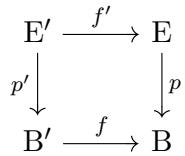
\includegraphics[keepaspectratio]{images/part003_c1a9b5e7.jpg}}

为一个笛卡尔方块。我们假设映射 f 是逆紧、分离且满射的，并作出下列假设之一：

\begin{enumerate}
\def\labelenumi{(\roman{enumi})}
\item
  f 的纤维是局部连通的，且纤维方块 \(B^{\prime} \times_{B} B^{\prime}\) 是局部连通的。
\item
  \(f\) 的纤维是有限的，\(\Delta_{\mathrm{B}^{\prime}}\) 是 \(\mathrm{B}^{\prime}\times_{\mathrm{B}}\mathrm{B}^{\prime}\) 的对角线，且在 \(\mathrm{B}^{\prime}\times_{\mathrm{B}}\mathrm{B}^{\prime}\) 中是开集，并且 \(\mathrm{B}^{\prime}\times_{\mathrm{B}}\mathrm{B}^{\prime} - \Delta_{\mathrm{B}^{\prime}}\) 是局部连通空间。
\end{enumerate}

那么，若 \((\mathrm{E}^{\prime}, p^{\prime})\) 是覆叠，\((\mathrm{E}, p)\) 也是覆叠。

由于映射 \(f\) 是万有严格的（I, 第~20~页，推论），映射 \(p\) 是平展的（I, 第~31~页，命题 8）且分离的（I, 第~27~页，命题 4）。不妨设 \(\mathrm{E}' = \mathrm{B}' \times_{\mathrm{B}} \mathrm{E}\)。

设 \(a\) 是 B 中一点；目标是证明点 \(a\) 有一个邻域 W，使得 W-空间 \((\mathrm{E_W}, p_{\mathrm{W}})\) 是可平凡化的覆叠。令 \(\mathrm{B}_a^\prime = f^{-1}(a)\)，并令 \(\mathrm{E}_a^\prime = (p')^{-1}(\mathrm{E}_a)\)。映射 \(t_a: \mathrm{E}_a^\prime \to \mathrm{B}_a^\prime \times \mathrm{E}_a\) 由 \(t_a(y) = (p'(y), f'(y))\) 定义，是一个 \(\mathrm{B}_a^\prime\)-同构（I, 第~9~页，命题 4），因此 \(\mathrm{E}_a^\prime\) 是 \(\mathrm{B}_a^\prime\) 的可平凡化覆叠，而 \(t_a\) 是此覆叠的平凡化。

证明存在一个邻域 \(V'\)，它是 \(B'_{a}\) 在 \(B'\) 中的邻域，以及覆叠（\(E_{V'}', p_{V'}\)）的一个连续平凡化 t，使其延拓 \(t_{a}\)。在假设（ii）下，\(B'_{a}\) 是有限的，且其中各点有两两不交的开邻域，在这些邻域上覆叠 \(E'\) 可平凡化，故此情形下断言成立。在假设（i）下，\(B'_{a}\) 是局部连通的，B' 也是如此（IV, 第~390~页，引理 1）；由于映射 f 逆紧且分离，\(B'_{a}\) 是紧的，且任意两个不同的点在 B' 中有不交邻域，从而偶对（B', \(B'_{a}\)）满足性质（PCV）（I, 第~37~页，引理 1）。因此断言由 I, 第~90~页推论 2 得出。

由于 \(f\) 逆紧，存在一个邻域 \(V\)，它是 \(a\) 在 \(B\) 中的邻域，使得 \(V'\) 包含 \(f^{-1}(V)\)（I, 第~75~页，引理）。因此不妨设 \(V' = f^{-1}(V)\)。

给 \(V'\)-空间 \(V' \times E_{a}\) 和 \(E_{V'}' = V' \times_{B} E\) 赋予关于 \(f_{V}: V' \to V\) 的规范下降数据。我们要证明，可能缩小 V 和 \(V'\) 后，刚定义的 \(V'\)-空间同构 \(t: E_{V'}' \to V' \times E_{a}\) 与下降数据相容，即有 \(t(b_{1}', x) = t(b_{2}', x)\)，只要 \((b_{1}', b_{2}') \in V' \times_{V} V'\) 且 \(x \in E_{f(b_{1}')}\)。记 \(\widetilde{t}\) 为映射 \(pr_{2} \circ t: E_{V'}' \to E_{a}\)。

令 \(V'' = V' \times_{V} V'\)；通过第一投影将其视为 \(V'\)-空间。映射 \(((b_{1}', b_{2}'), x) \mapsto ((b_{1}', b_{2}'), (b_{1}', x))\)，从 \(V'' \times_{V} E\) 到 \(V'' \times_{V'} E'\)，是 \(V''\)-空间的同构；这说明 \(V'' \times_{V} E\) 是 \(V''\) 的覆叠。

对 \(i=1,2\)，定义映射 \(u_{i}\colon V^{\prime\prime}\times_{V}E\to V^{\prime\prime}\times E_{a}\)，令 \(u_{i}(b_{1}^{\prime},b_{2}^{\prime},x)=(b_{1}^{\prime},b_{2}^{\prime},\widetilde{t}(b_{i}^{\prime},x))\)；它们是覆叠 \(V^{\prime\prime}\times_{V}E\) 的平凡化。令 \(W^{\prime\prime}\) 为点 \(w\in V^{\prime\prime}\) 的集合，在这些点上平凡化 \(u_{1}\) 和 \(u_{2}\) 重合；它包含 \(B_{a}^{\prime}\times B_{a}^{\prime}\)，也包含对角线 \(\Delta_{V'}\)。证明 \(W^{\prime\prime}\) 是 \(B_{a}^{\prime}\times B_{a}^{\prime}\) 的一个邻域。在假设（i）下，这由 I, 第~80~页推论 2 得出，因为 \(B^{\prime}\times B^{\prime}\) 是局部连通的。在假设（ii）下，\(W^{\prime\prime}\) 包含 \((B_{a}^{\prime}\times B_{a}^{\prime})-\Delta_{B_{a}^{\prime}}\) 在 \((B^{\prime}\times_{B}B^{\prime})-\Delta_{B^{\prime}}\) 中的一个邻域，因为这个集合是局部连通的（同上）。由于 \(\Delta_{V'}\) 在 \(B^{\prime}\times_{B}B^{\prime}\) 中开，\(W^{\prime\prime}\) 是 \(B_{a}^{\prime}\times B_{a}^{\prime}\) 在 \(V^{\prime\prime}\) 中的一个邻域。

由于 \(f\) 逆紧，规范映射 \(f''\) 将 \(\mathrm{B}' \times_{\mathrm{B}} \mathrm{B}'\) 映到 B，并且是逆紧的，因为它是投影 \(\mathrm{pr}_{1} \colon \mathrm{B}' \times_{\mathrm{B}} \mathrm{B}' \to \mathrm{B}'\) 与映射 \(f\) 的复合。

根据 I, 第~75~页的引理，存在 V 中 a 的一个邻域 W，使得 \((f'')^{-1}(\mathrm{W})\) 包含于 \(W''\)；令 \(W'=(f')^{-1}(\mathrm{W})\)，它是 \(V'\) 的子集，且平展空间同构 \(t: E_{W'}' \to W' \times E_a\) 与关于映射 \(f_W: W' \to W\) 的规范下降数据相容。根据推论（IV, 第~388~页），

W-平展空间 \(E_{W}\) 和 \(W \times E_{a}\) 同构。特别地，\(E_{W}\) 是可平凡化覆叠，命题得证。

推论 1. --- 设 E 和 B 是拓扑空间，\(p\colon\mathrm{E}\to\mathrm{B}\) 是连续映射，且 \((\mathrm{A}_{i})_{i\in\mathrm{I}}\) 是 B 的局部有限闭覆盖，使得对每一对 \((i,j)\in\mathrm{I}\times\mathrm{I}, i\neq j\)，交集 \(\mathrm{A}_{i}\cap\mathrm{A}_{j}\) 是局部连通空间。那么，B-空间 \((\mathrm{E},p)\) 是覆叠的必要且充分条件是：对每个 \(i\in\mathrm{I}\)，\(\mathrm{A}_{i} \)-空间 \((p^{-1}(\mathrm{A}_{i}),p_{\mathrm{A}_{i}})\) 是 \(\mathrm{A}_{i}\) 的覆叠。

这个条件是必要的（参见 I, 第~69~页）。反之，令 B' 为族 \((\mathrm{A}_{i})_{i\in\mathrm{I}}\) 的拓扑和空间，令 \(f\colon B'\to B\) 为规范映射。映射 f 是闭的（TG, I, 第~6~页，命题 4）、分离的（I, 第~27~页，注 5），具有有限纤维，因而是逆紧的（TG, I, 第~75~页，定理 1）；它还是满射。对角线 \(\Delta_{B'}\) 等于 \(\bigcup_{i\in I}A_{i}\times_{B}A_{i}\)，所以在 \(B'\times_{B}B'\) 中是开集。最后，空间 \((\mathrm{B}'\times_{\mathrm{B}}\mathrm{B}')-\Delta_{\mathrm{B'}}\) 同胚于族 \((\mathrm{A}_{i}\cap\mathrm{A}_{j})\)、\((i,j)\in\mathrm{I}\times\mathrm{I}\)、\(i\neq j\) 的和空间；因而是局部连通的。命题 6 的假设（ii）得到满足。若对每个 i，\(p^{-1}(\mathrm{A}_{i})\) 是 \(A_{i}\) 的覆叠，则 \(E'\) 是 \(B'\) 的覆叠，故 E 是 B 的覆叠。

推论 2. --- 设 X 和 Y 是拓扑空间，设 \(f\colon X \to Y\) 是逆紧、分离且满射的映射。此外，假设下列假设之一成立：

\begin{enumerate}
\def\labelenumi{(\roman{enumi})}
\item
  f 的纤维以及空间 \(X\times_Y X\) 都是局部连通的；
\item
  \(f\) 的纤维是有限的，\(\Delta_{\mathrm{X}}\) 是 \(\mathrm{X} \times_{\mathrm{Y}} \mathrm{X}\) 的对角线，并且在 \(\mathrm{X} \times_{\mathrm{Y}} \mathrm{X}\) 中是开集，空间 \((\mathrm{X} \times_{\mathrm{Y}} \mathrm{X}) - \Delta_{\mathrm{X}}\) 是局部连通的。于是，关于 \(f\) 在 \(\mathrm{X}\) 的覆叠上的每个下降数据都是有效的，且商空间是 \(\mathrm{Y}\) 的覆叠。
\end{enumerate}

设 Z 是 X 的覆叠，\(\tau\) 是关于 f 在 Z 上的下降数据。根据命题 5（IV, 第~389~页），下降数据 \(\tau\) 是有效的，换言之，图表

\pandocbounded{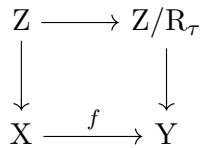
\includegraphics[keepaspectratio]{images/part003_fd3d7e4d.jpg}}

是笛卡尔方形。于是命题 6（IV, 第~391~页）的假设得到满足。因此，\(Z/R_{\tau}\) 是 Y 的覆叠。

命题 7. --- 设 X 和 Y 是拓扑空间，设 \(f: X \to Y\) 是连续且满射的映射。假设 Y 是可解圈的，且映射 f 是开映射并具有道路提升性质。那么，关于 f 在 X 的覆叠上的每个下降数据都是有效的，且商空间是 Y 的覆叠。

设 \((Z,p)\) 是 X 的覆叠，\(\tau\) 是关于 f 在 Z 上的下降数据。由于映射 f 满射且开，根据 IV, 第~389~页命题 5，下降数据 \(\tau\) 是有效的。令 \(T = Y/R_{\tau}\) 表示商 Y-空间；其投影 q 是平展的（同上），也是分离的（I, 第~27~页，命题 4）。

根据假设，映射 f 具有道路提升性质；映射 p 也有，因为 Z 是 X 的覆叠（III, 第~302~页，命题 3 的推论 2）。因此映射 \(p \circ f\) 也具有这一性质，从而映射 q 也有。于是（参见 IV, 第~341~页，注 2），T 是 Y 的覆叠。命题得证。

注。--- 设 X 和 Y 是拓扑空间，设 \(f: X \rightarrow Y\) 是映射。要使关于 f 在 X 的覆叠上的每个下降数据都有效且商空间是 Y 的覆叠，必要条件是 f 严格，并且 \(f(X)\) 是 X 的开闭子集。

事实上，将 X-空间 X 识别为 \(X \times_{Y} Y\)，并赋予它关于 f 的规范下降数据。商空间可识别为 \(f(\mathrm{X})\)，它带有由 f 定义的等价关系下从 X 的拓扑得到的商拓扑。若这是 Y 的覆叠，则空间 \(f(\mathrm{X})\) 可识别为 Y 的开闭子集，而映射 f 是严格的。

\subsection{群胚的下降}

设 X 和 Y 是拓扑空间，设 \(f\colon\mathrm{X}\to\mathrm{Y}\) 是连续映射。设 \(p_{1}\) 和 \(p_{2}\) 是 \(\mathrm{X}\times_{\mathrm{Y}}\mathrm{X}\) 到 X 的两个投影，\(\operatorname{Coeg}(f)\) 是群胚态射对 \((\varpi(p_{1}),\varpi(p_{2}))\) 的余均衡群胚，这两个态射从 \(\varpi(\mathrm{X}\times_{\mathrm{Y}}\mathrm{X})\) 到 \(\varpi(\mathrm{X})\)，而 \(\gamma\colon\varpi(\mathrm{X})\to\operatorname{Coeg}(f)\) 是规范群胚态射（II, 第~199~页，定义 2）。由于 \(f\circ p_{1}=f\circ p_{2}\)，有 \(\varpi(f)\circ\varpi(p_{1})=\varpi(f)\circ\varpi(p_{2})\)。因此根据余均衡子的泛性质（II, 第~199~页，命题 3），存在唯一的群胚态射 \(\varpi'(f)\colon\operatorname{Coeg}(f)\to\varpi(\mathrm{Y})\)，使得 \(\varpi(f)=\varpi'(f)\circ\gamma\)。

Coeg(f) 的顶点集是集合 X = Vert( \(\varpi(X)\) ) 按 f 定义的等价关系所得的商集（II, 第~200~页，注 1）。它可识别为 f(X)。

命题 8. --- 设 X 和 Y 是非空拓扑空间，f 是从 X 到 Y 的连续映射。假设 X 局部道路连通，Y 连通，且 f 严格且满射。那么群胚 Coeg(f) 是传递的。

设 \(\Gamma\) 是这样的箭图：其顶点集为 X，箭集为 \(\mathrm{Fl}(\varpi(\mathrm{X}))\) 与 \(\mathrm{X}\times_{\mathrm{Y}}\mathrm{X}\) 的不交并；源映射和目标映射是 \(\varpi(\mathrm{X})\) 的源映射和目标映射（作用于 \(\mathrm{Fl}(\varpi(\mathrm{X}))\)），以及映射 \(p_1\) 和 \(p_2\)（作用于 \(\mathrm{X}\times_{\mathrm{Y}}\mathrm{X}\)）。根据对 \((\varpi(\mathrm{pr}_1), \varpi(\mathrm{pr}_2))\) 的框架的定义（II, 第~185~页，定义 3）以及 II, 第~200~页注 2，\(\operatorname{Coeg}(f)\) 的轨道集可识别为箭图 \(\Gamma\) 的连通分支集。由于空间 X 非空，只需证明图 \(\Gamma\) 是连通的。

\(\Gamma\) 的连通分支关于等价关系“存在道路连接 \(x\) 与 \(x'\)”是饱和的，因此由于 X 局部道路连通，它们在 X 中是开集。于是它们也是闭集。它们关于 f 定义的等价关系 R 也是饱和的。根据假设，映射 f 诱导出从 X/R 到 Y 的同胚，所以每个 \(\Gamma\) 的连通分支在 f 下的像都是 Y 的开闭子集；由于空间 Y 连通，这个像必为 Y。

设 C 是 \(\Gamma\) 的一个连通分支，设 \(x\) 是 X 中一点。根据前述内容，存在 \(x' \in \mathrm{C}\)，使得 \(f(x') = f(x)\)。根据箭图 \(\Gamma\) 的定义，有 \(x' \in \mathrm{C}\)。因此 \(\mathrm{C} = \mathrm{X}\)，箭图 \(\Gamma\) 从而是连通的。

命题 9. --- 设 X 和 Y 是拓扑空间，f 是从 X 到 Y 的连续映射。假设 X 局部道路连通，Y 是可解圈的，且映射 f 严格且满射。那么，群胚 \(\varpi(\mathrm{Y})\) 由 \(\varpi(\mathrm{X})\) 在 \(\varpi(f)\) 下的像生成。

不妨设空间 X 和 Y 非空。令 G 为 \(\varpi(\mathrm{Y})\) 中由 \(\varpi(\mathrm{X})\) 在 \(\varpi(f)\) 下的像生成的子群胚。由于映射 f 满射，G 的顶点集等于 Y。根据命题 8，\(\operatorname{Coeg}(f)\) 是传递群胚。由于 \(\varpi'(f)\) 在顶点上诱导恒等，\(\operatorname{Coeg}(f)\) 在 \(\varpi'(f)\) 下的像是 \(\varpi(\mathrm{Y})\) 的传递子群胚。\(\varpi(\mathrm{X})\) 在 \(\gamma\) 下的像生成 \(\operatorname{Coeg}(f)\)（II, 第~200~页，推论）；由于有 \(\varpi(f) = \varpi'(f) \circ \gamma\)，群胚 G 是传递的。

设 \(y_{0}\) 是 Y 中一点，令 H 表示子群 \(G_{y_{0}}\)，它是 \(\pi_{1}(Y, y_{0})\) 的子群。根据 IV, 第~342~页定理 1，存在 Y 的连通覆叠（T, p）以及一点 \(t_{0}\)，它属于纤维 \(T_{y_{0}}\)，且其固定子为 H。

若 \(x\) 是 X 中一点，则集合 \(\mathrm{Fl}_{y_0,f(x)}(\mathrm{G})\) 非空，因为 G 是传递的。对于 \(u\in \mathrm{Fl}_{y_0,f(x)}(\mathrm{G})\)，点 \(t_0\cdot u\) 是纤维 \(\mathrm{T}_{f(x)}\) 中的一点，并且与 \(u\) 无关，因为群 H（G 在 \(y_0\) 处的各向同性群）固定 \(t_0\)。将此点记为 \(\sigma (x)\)；将由此定义的映射 \(\sigma \colon \mathrm{X}\to \mathrm{T}\) 记为，并令 \(s\colon \mathrm{X}\to \mathrm{X}\times_{\mathrm{Y}}\mathrm{T}\) 为映射 \(x\mapsto (x,\sigma (x))\)。按构造，映射 s 与 \(\varpi (\mathrm{X})\) 在 X 和 \(\mathrm{X}\times_{\mathrm{Y}}\mathrm{T}\) 上的规范作用相容。由 III, 第~312~页引理 1，s 是连续的。因此映射 \(\sigma\) 连续；此外，由于 \(\sigma (x)\) 只依赖于 \(f(x)\)，它与 f 定义的等价关系相容。由于 f 严格且满射，存在唯一连续映射 \(\overline{\sigma}\colon \mathrm{Y}\to \mathrm{T}\)，使得 \(\overline{\sigma}\circ f = \sigma\)，所以覆叠 T 有截面。由于 T 连通，映射 \(p\colon \mathrm{T}\to \mathrm{Y}\) 是同胚（I, 第~31~页，命题 6 的推论 4），并且 \(\mathrm{H} = \pi_1(\mathrm{Y},y_0)\)，从而 \(\mathrm{G}_{y_0} = \pi_1(\mathrm{Y},y_0)\)。由于 G 传递，得到 \(\mathrm{G} = \varpi (\mathrm{Y})\)。

命题 10. --- 设 X 和 Y 是拓扑空间，f 是从 X 到 Y 的连续映射。假设空间 X 是可解圈的，空间 \(X\times_{Y}X\) 局部道路连通，并且关于 f 在 X 的覆叠上的每个下降数据都是有效的，商空间是 Y 的覆叠。那么群胚态射 \(\varpi'(f)\) 从 Coeg(f) 到 \(\varpi(Y)\)，是单射。

在命题的假设下，\(f\) 是严格的（IV, 第~394~页，注）；此外不妨设它是满射的。

引理 2. --- 保持命题的记号和假设。设 T 是一个集合，赋予它相对于映射 q: T → Y 的群胚 Coeg(f) 作用。那么 T 上存在唯一拓扑，使得 q 使 T 成为 Y 的覆叠，并且对于以 X 中 c 为起点的每个道路类以及 T 中每个点 t，都有 \(t \cdot \gamma(c) = t \cdot f_{*}(c)\)。特别地，Coeg(f) 在 T 上的作用可通过群胚 \(\varpi(Y)\) 的作用分解。

这种 T 上拓扑的唯一性由 III, 第~312~页引理 1 得出；证明其存在性。给集合 \(X\times_{Y}T\) 赋予 \(\varpi(\mathrm{X})\) 的作用，规定 \((x,t)\cdot u=(x\cdot u,t\cdot\gamma(u))\)，其中 \((x,t)\in\mathrm{X}\times_{\mathrm{Y}}\mathrm{T}\)，且 u 是 \(\varpi(\mathrm{X})\) 中源为 x 的每个箭。由于空间 X 是可解圈的，此作用没有局部单值性（III, 第~313~页，注）。因此，在集合 \(X\times_{Y}T\) 上存在唯一拓扑，使 X-空间 \((\mathrm{X}\times_{\mathrm{Y}}\mathrm{T},\mathrm{pr}_{1})\) 成为 X 的覆叠，并使 \(\varpi(\mathrm{X})\) 在此覆叠上的规范作用与给定作用重合（III, 第~313~页，命题 3）。记此覆叠为 \((Z,p)\)。证明映射 \(\tau: ((x_{1},t),x_{2})\mapsto(x_{2},t)\)，从 \(Z\times_{Y}X\) 到 Z，是关于映射 f 在 Z 上的下降数据。只需验证它连续，IV, 第~382~页定义 1 的其他条件显然成立。

映射 \(\tau\) 是映射 \(\mathrm{pr}_2\colon Z\times_Y X\to X\) 到覆叠 \(Z\)（其底空间为 \(X\)）的提升。由于空间 \(X\times_Y X\) 局部道路连通，作为它的覆叠的空间 \(Z\times_Y X\) 也局部道路连通。根据推论（III, 第~269~页），要证明映射 \(\tau\) 连续，只需证明它沿道路连续。

设 \(\widetilde{c} = ((c,g),c')\) 是 \(Z\times_{Y}X\) 中的一条道路，证明映射 \(\tau \circ \widetilde{c}\colon t\mapsto (c'(t),g(t))\) 从 I 到 Z 连续。对于每个 \(s\in [0,1]\)，记 \(c_s\) 和 \(c_s'\) 为 X 中分别由 \(t\mapsto c(st)\) 和 \(t\mapsto c'(st)\) 定义的道路。对于所有 \(s\in [0,1]\)，于是有 \(c(s) = c(0)\cdot [c_s]\)、\(c'(s) = c'(0)\cdot [c_s']\) 以及 \((c,g)(s) = (c(0),g(0))\cdot [c_s]\)，其中 \([u]\) 表示道路 u 的严格同伦类（III, 第~304~页，注）。映射 \(t\mapsto (c_s(t),c_s'(t))\) 是 \(X\times_{Y}X\) 中的一条道路；根据余均衡群胚 Coeg(f) 的定义，有 \(\gamma ([c_s]) = \gamma ([c_s'])\)，并且 \(g(s) = g(0)\cdot \gamma ([c_s]) = g(0)\cdot \gamma ([c_s'])\)。根据 \(\varpi (X)\) 在 Z 上的作用定义，因而有

\[
\begin{array}{r} (\tau \circ \widetilde {c}) (s) = (c ^ {\prime} (s), g (s)) = (c ^ {\prime} (0) \cdot [ c _ {s} ^ {\prime} ], g (0) \cdot \gamma ([ c _ {s} ^ {\prime} ])) \\ = (c ^ {\prime} (0), g (0)) \cdot [ c _ {s} ^ {\prime} ] = (\tau \circ \widetilde {c}) (0) \cdot [ c _ {s} ^ {\prime} ]. \end{array}
\]

这说明 \(\tau \circ \widetilde{c}\) 是道路 \(c'\) 到 Z 的连续提升（同上）。因此，映射 \(\tau\) 沿道路连续，因而连续；它是 X-空间 Z 关于 \(f\) 的下降数据。

记 \(R_{\tau}\) 为下降数据 \(\tau\) 定义的等价关系。由于映射 f 满射，映射 \(pr_{2}: Z \to T\) 通过取商诱导出从 \(Z/R_{\tau}\) 到 T 的双射。通过结构传递，将由 \(Z/R_{\tau}\) 的拓扑得到的拓扑赋予 T，使得 \((T,q)\) 成为 Y-空间。根据假设，T 因而是 Y 的覆叠，且图表

\[
\begin{array}{c} \mathrm{Z} \xrightarrow {\mathrm{pr} _ {2}} \mathrm{T} \\ p \Big \downarrow \qquad \qquad \qquad \qquad \Big \downarrow q \\ \mathrm{X} \xrightarrow {f} \mathrm{Y} \end{array}
\]

是笛卡尔方形。

设 \((x,t)\) 是 Z 中一点，设 c 是 X 中以 x 为起点的一条道路，并设 \(\widetilde{c}\) 是以 \((x,t)\) 为起点的 c 到 Z 的连续提升。道路 \(pr_{2} \circ \widetilde{c}\) 是道路 \(f \circ c\) 在 Y 中以 t 为起点的提升，因此 \(t \cdot \gamma([c]) = t \cdot [f \circ c] = t \cdot f_{*}([c])\)。引理得证。

现在证明命题。设 \(u\) 和 \(v\) 是 Coeg( \(f\) ) 的两个箭，它们在 \(\varpi(Y)\) 中的像相等。由于群胚态射 \(\varpi'(f)\) 在顶点集上是恒等的，箭 \(u\) 和 \(v\) 有相同的起点和终点。记 \(y\) 为 \(u\) 的起点；令 T 为 Coeg( \(f\) ) 中以 y 为源的箭集，并令 \(q: \mathrm{T} \to \mathrm{Y}\) 为目标映射在 T 上的限制。群胚 Coeg( \(f\) ) 关于 \(q\) 通过右合成作用于集合 T。根据引理 2，\(u\) 和 \(v\) 在 T 上的作用相同。因此有 \(u = e_y \cdot u = e_y \cdot v = v\)。这证明群胚态射 \(\varpi'(f)\) 是单射。

定理 1. --- 设 X 和 Y 是拓扑空间，设 \(f: X \to Y\) 是连续且满射的映射。假设空间 X 和 Y 都是可解圈的。最后，假设下列性质之一成立：

\begin{enumerate}
\def\labelenumi{(\roman{enumi})}
\item
  映射 f 逆紧、分离，具有局部连通的纤维，且空间 \(X\times_{Y}X\) 局部道路连通；
\item
  映射 f 逆紧、分离，具有有限纤维，对角线 \(\Delta_{X}\) 在 \(X \times_{Y} X\) 中是开集，且其补集是局部连通的；
\item
  映射 f 是开映射并具有道路提升性质。
\end{enumerate}

那么，群胚态射 \(\varpi'(f)\) 是从群胚 Coeg(f) 到庞加莱群胚 \(\varpi(Y)\) 的同构。

首先注意，在这些假设下，映射 \(f\) 是满射且严格的（I, 第~18~页，例 2）。此外，关于 \(f\) 在 X 的覆叠上的每个下降数据都是有效的，商空间是 Y 的覆叠；这在假设（i）和（ii）下由 IV, 第~393~页命题 4 的推论 2 得出，在假设（iii）下由 IV, 第~394~页命题 7 得出。根据命题 10，群胚态射 \(\varpi'(f)\) 因而是单射，且其像是 \(\varpi(Y)\) 的子群胚。

根据 IV, 第~395~页命题 9，在假设（i）和（ii）下，此像等于 \(\varpi(\mathrm{Y})\)；在假设（iii）下也如此，因为此时群胚态射 \(\varpi(f)\) 是满射的。

因此，\(\varpi'(f)\) 是同构。

例。--- 下面是两个满足定理 1 假设的例子。

\begin{enumerate}
\def\labelenumi{\arabic{enumi})}
\item
  设 Y 是可解圈拓扑空间。设 \((\mathrm{A}_{i})_{i\in\mathrm{I}}\) 是由闭集构成的 Y 的局部有限覆盖。假设对每个 \(i\in I\)，空间 \(A_{i}\) 是可解圈的，并且对每一对 \((i,j)\in\mathrm{I}\times\mathrm{I}\)，空间 \(A_{i}\cap A_{j}\) 局部道路连通。可以取 X 为族 \((\mathrm{A}_{i})_{i\in\mathrm{I}}\) 的和空间，取 \(f:X\to Y\) 为由规范嵌入族导出的映射。
\item
  设 G 是作用在可解圈拓扑空间 X 上的离散群，且作用是适当的；令 Y = X/G，并令 \(f: X \to Y\) 为规范映射。它是开映射（TG, III, 第~10~页，引理 2），并根据 III, 第~287~页定理 4 具有道路提升性质。根据 IV, 第~349~页命题 8 b)，空间 Y 是可解圈的。由从 G × X 到 \(X\times X\) 的映射 \((g, x) \mapsto (g \cdot x, x)\) 给出的映射是逆紧的，因而严格（I, 第~18~页，例 2），且其像是 \(X\times_{Y}X\)。于是根据 III, 第~261~页命题 8，\(X\times_{Y}X\) 局部道路连通。
\end{enumerate}

\subsection{通过平展且满射的映射下降}

设 X 和 Y 是拓扑空间，f 是从 X 到 Y 的连续映射。沿用前一节的记号。

定理 2. --- 假设 Y 的每一点都有一个邻域，在其上存在映射 f 的连续截面。那么，群胚态射 \(\varpi'(f)\) 是从 \(\operatorname{Coeg}(f)\) 到 \(\varpi(Y)\) 的同构。

根据假设，存在由开集构成的 Y 的覆盖 \((\mathrm{U}_{j})_{j\in\mathrm{J}}\)，并且对每个 \(j\in J\)，有连续截面 \(s_{j}\)，它是 \(f_{U_{j}}\) 的截面。

若 \(c\) 是 X 中的一条道路，我们将 \([c]\) 记为它在 \(\varpi(X)\) 中的严格同伦类，将 \(\{c\}\) 记为 \([c]\) 在 \(\operatorname{Coeg}(f)\) 中经群胚态射 \(\gamma\) 得到的像。若 \(c\) 和 \(c'\) 是 X 中的两条道路，则 \(\{c\}\) 和 \(\{c'\}\) 在 \(\operatorname{Coeg}(f)\) 中可合成，当且仅当道路 \(f \circ c\) 和 \(f \circ c'\) 在 Y 中可首尾相接。

设 \(c'\) 是 Y 中的一条道路。根据 III, 第~272~页引理 4，将其应用于紧空间 I 以及 I 的覆盖 \(((c')^{-1}(\mathrm{U}_j))_{j\in \mathrm{J}}\)，存在整数 \(n\)，使得对每个整数 \(k\)，若满足 \(1\leqslant k\leqslant n\)，则区间 \([\frac{k - 1}{n},\frac{k}{n}]\) 在 \(c'\) 下的像包含于某个开集 \(\mathrm{U}_{j(k)}\) 中。对每个整数 \(k\)，若 \(1\leqslant k\leqslant n\)，令 \(c_k'\) 为 Y 中由 \(s\mapsto c'(\frac{k + s - 1}{n})\) 定义的道路；有 \([c'] = [c_1'][c_2']\ldots [c_n']\)（参见 III, 第~291~页，注 1），且 \(c'\) 就是记作 \(c_1' * c_2' * \dots * c_n'\) 的道路。对所有 \(k\in \{1,\ldots ,n\}\)，记 \(c_k\) 为 X 中的道路 \(s_{j(k)}\circ c_k'\)，并置 \(\{c_k\} = \gamma ([c_k])\)。由于对每个 \(k\)，道路 \(c_{k - 1}' = f\circ c_{k - 1}\) 和 \(c_k' = f\circ c_k\) 可首尾相接，序列 \((\{c_1\} ,\ldots ,\{c_n\})\) 在 \(\operatorname{Coeg}(f)\) 中可合成。由构造，

\[
\begin{array}{r l} & {\varpi^ {\prime} (f) (\{c _ {1} \} \ldots \{c _ {n} \}) = \varpi^ {\prime} (f) (\{c _ {1} \}) \ldots \varpi^ {\prime} (f) (\{c _ {n} \})} \\ & {\qquad = \varpi (f) ([ c _ {1} ]) \ldots \varpi (f) ([ c _ {n} ])} \\ & {\qquad = [ f \circ c _ {1} ] \ldots [ f \circ c _ {n} ]} \\ & {\qquad = [ c _ {1} ^ {\prime} ] * \dots * [ c _ {n} ^ {\prime} ] = [ c ^ {\prime} ],} \end{array}
\]

这证明群胚态射 \(\varpi'(f)\) 是满射。

设 \(u\) 和 \(v\) 是 \(\operatorname{Coeg}(f)\) 的箭。由于群胚 \(\operatorname{Coeg}(f)\) 由 \(\varpi(\mathrm{X})\) 的像生成（II, 第~200~页，推论），存在 X 中道路的有限序列 \((c_1, \ldots, c_n)\) 和 \((d_1, \ldots, d_n)\)，使得 \(u = \{c_1\} \ldots \{c_n\}\) 且 \(v = \{d_1\} \ldots \{d_n\}\)。道路 \((f \circ c_1, \ldots, f \circ c_n)\) 在 Y 中可首尾相接，并且有 \(\varpi'(f)(u) = [(f \circ c_1)] \ldots [(f \circ c_n)]\)；同样，\(\varpi'(f)(v) = [(f \circ d_1)] \ldots [(f \circ d_n)]\)。

假设有 \(\varpi'(f)(u) = \varpi'(f)(v)\)。于是存在严格同伦 \(\sigma\)，连接 \((f \circ c_1) * \cdots * (f \circ c_n)\) 与 \((f \circ d_1) * \cdots * (f \circ d_n)\)。根据 III, 第~272~页引理 4，将其应用于紧空间 \(\mathbf{I} \times \mathbf{I}\) 以及覆盖 \((\bar{\sigma}^{-1}(\mathrm{U}_i))_{i \in \mathrm{I}}\) 的空间 \(\mathbf{I} \times \mathbf{I}\)，存在整数 \(m \geqslant 1\)，使得对每一对整数 \((j,k)\)，若满足 \(1 \leqslant j \leqslant m\) 且 \(1 \leqslant k \leqslant m\)，则区间积 \([\frac{j-1}{m}, \frac{j}{m}] \times [\frac{k-1}{m}, \frac{k}{m}]\) 在 \(\sigma\) 下的像包含于某个开集 \(U_{i(j,k)}\) 中，该开集属于覆盖 \((\mathrm{U}_{i})_{i \in \mathrm{I}}\)。

X 中每条道路 c 都形如 \(c_{1}*\cdots*c_{m}\)，其中 \(c_{k}\) 是由 \(t\mapsto c(\frac{k-1+t}{m})\) 定义的道路。如有必要，将整数 m 和 n 换成它们的乘积 mn，因此可以假设 m=n。

对于每一对整数 \((j,k)\)（属于 \(\{1,\ldots ,n\}\)）以及每一对 \((s,t)\in\) \(\mathbf{I}\times \mathbf{I}\)，置

\[
\sigma_ {j, k} (s, t) = s _ {i (j, k)} \circ \sigma \left(\frac {s + j - 1}{n}, \frac {t + k - 1}{n}\right).
\]

对于 \(t \in \mathbf{I}\)，再置 \(h_{j,k}^{0}(t) = \sigma_{j,k}(t,0)\)、\(h_{j,k}^{1}(t) = \sigma_{j,k}(t,1)\)、\(v_{j,k}^{0}(t) = \sigma_{j,k}(0,t)\) 以及 \(v_{j,k}^{1}(t) = \sigma_{j,k}(1,t)\)。根据 III, 第~295~页引理 1，道路 \(h_{j,k}^{0} * v_{j,k}^{1}\) 和 \(v_{j,k}^{0} * h_{j,k}^{1}\) 严格同伦，因此有关系

\[
[ h _ {j, k} ^ {0} ] [ v _ {j, k} ^ {1} ] = [ v _ {j, k} ^ {0} ] [ h _ {j, k} ^ {1} ]\tag{2}
\]

在 \(\varpi(\mathrm{X})\) 上，对每一对 \((j,k) \in \{1, \ldots, n\}^2\) 都成立。另一方面，对每一对整数 \((j,k)\)，若 \(2 \leqslant j \leqslant n\) 且 \(1 \leqslant k \leqslant n\)，有 \(f \circ v_{j,k}^0 = f \circ v_{j-1,k}^1\)，因此有关系

\[
\{v _ {j, k} ^ {0} \} = \{v _ {j - 1, k} ^ {1} \}\tag{3}
\]

在 Coeg(f) 中。类似地，对每一对整数 \((j,k)\)，若 \(1 \leqslant j \leqslant n\) 且 \(2 \leqslant k \leqslant n\)，有

\[
\{h _ {j, k} ^ {0} \} = \{h _ {j, k - 1} ^ {1} \}.\tag{4}
\]

对于 \(j \in \{1, \ldots, n\}\)，道路 \(f \circ c_j\) 和 \(f \circ h_{j,1}^0\) 重合。根据余均衡子 Coeg(f) 的定义，因此有 \(\{c_j\} = \{h_{j,1}^0\}\)。同样，对每个 \(j \in \{1, \ldots, n\}\)，有 \(\{d_j\} = \{h_{j,n}^1\}\)。因此有如下关系

\[
u = \{h _ {1, 1} ^ {0} \} \dots \{h _ {n, 1} ^ {0} \}, \quad v = \{h _ {1, n} ^ {1} \} \dots \{h _ {n, n} ^ {1} \}.
\]

根据下面的引理 3，有

\[
\{h _ {1, 1} ^ {0} \} \dots \{h _ {1, n} ^ {0} \} \{v _ {1, n} ^ {1} \} \dots \{v _ {n, n} ^ {1} \} = \{v _ {1, 1} ^ {0} \} \dots \{v _ {n, 1} ^ {0} \} \{h _ {n, 1} ^ {1} \} \dots \{h _ {n, n} ^ {1} \}.
\]

由于道路 \(t \mapsto \sigma(0,t)\) 和 \(t \mapsto \sigma(1,t)\) 是常值，对 \(1 \leqslant k \leqslant n\)，有 \(\{v_{1,k}^{0}\} = e_{a}\) 且 \(\{v_{n,k}^{1}\} = e_{b}\)，其中 \(a,b \in Y\) 是箭 \(u\) 和 \(v\) 的起点和终点，它们属于群胚 Coeg( \(f\) )。因此有等式

\[
\{h _ {1, 1} ^ {0} \} \dots \{h _ {1, n} ^ {0} \} = \{h _ {n, 1} ^ {0} \} \dots \{h _ {n, n} ^ {1} \},
\]

即 u = v。

引理 3. --- 设 G 是群胚，p、q 是满足 \(\geqslant 1\) 的整数。对于每一对整数 \((j, k)\)，若 \(0 \leqslant j \leqslant p\) 且 \(0 \leqslant k \leqslant q\)，令 \(x_{j,k}\) 为 G 的一个顶点；对于每一对整数 \((j, k)\)，若 \(1 \leqslant j \leqslant p\) 且 \(0 \leqslant k \leqslant q\)，令 \(h_{j,k}\) 为连接 \(x_{j-1,k}\) 与 \(x_{j,k}\) 的 G 的一个箭；对于每一对整数 \((j, k)\)，若 \(0 \leqslant j \leqslant p\) 且 \(1 \leqslant k \leqslant q\)，令 \(v_{j,k}\) 为连接 \(x_{j,k-1}\) 与 \(x_{j,k}\) 的 G 的一个箭。

假设对于每一对整数 \((j,k)\)，若 \(1 \leqslant j \leqslant p\) 且 \(1 \leqslant k \leqslant q\)，箭 \(v_{j-1,k}\) 和 \(h_{j,k}\) 可合成，箭 \(h_{j,k-1}\) 和 \(v_{j,k}\) 也可合成，并且有 \(v_{j-1,k}h_{j,k} = h_{j,k-1}v_{j,k}\)。那么，

\[
h _ {1, 0} h _ {2, 0} \dots h _ {p, 0} v _ {p, 1} v _ {p, 2} \dots v _ {p, q} = v _ {0, 1} v _ {0, 2} \dots v _ {0, q} h _ {1, q} h _ {2, q} \dots h _ {p, q}.
\]

先处理 q = 1 的特殊情形，并对 p 作归纳证明。若 p = 1，待证断言由假设得到验证；假设它对 p - 1 成立；于是有

\[
h _ {1, 0} h _ {2, 0} \dots h _ {p, 0} v _ {p, 1} = h _ {1, 0} h _ {2, 0} \dots h _ {p - 1, 0} v _ {p - 1, 1} h _ {p, 1} = v _ {0, 1} h _ {1, 1} \dots h _ {p, 1}
\]

根据归纳假设，从而得到 p 的关系。

现在对 q 作归纳证明。根据前述内容，q = 1 时命题成立；若对 q - 1 成立，则有

\[
h _ {1, 0} h _ {2, 0} \dots h _ {p, 0} v _ {p, 1} v _ {p, 2} \dots v _ {p, q} = v _ {0, 1} v _ {0, 2} \dots v _ {0, q - 1} h _ {1, q - 1} \dots h _ {p, q - 1} v _ {p, q}.
\]

根据 \(q = 1\) 的情形，有

\[
h _ {1, q - 1} \dots h _ {p, q - 1} v _ {p, q} = v _ {0, q} h _ {1, q} \dots h _ {p, q},
\]

从而得到所需关系。

例。--- 1) 当映射 f 平展且满射时，定理适用。

\begin{enumerate}
\def\labelenumi{\arabic{enumi})}
\setcounter{enumi}{1}
\tightlist
\item
  它也适用于如下情形：空间 X 是集合族 \((V_{i})_{i\in\mathrm{I}}\) 的和空间，其中这些 Y 的子集的内部覆盖 Y，且 f 是由每个 \(V_{i}\) 到 Y 的规范嵌入导出的映射。
\end{enumerate}

\subsection{商空间的庞加莱群胚}

设 X 是赋予离散群 G 连续作用的拓扑空间；令 Y = X/G，并将 \(f: X \to Y\) 记为规范映射。记 \(\lvert G\rvert\) 为群胚 \(\varpi(G)\)；其顶点集为 G；对于 \(g, g' \in G\)，存在从 g 到 \(g'\) 的唯一箭，当且仅当 \(g' = g\)，否则不存在。通过取基本群胚，作用 \(m: G \times X \to X\) 诱导出群胚态射 \(\varpi(m): \lvert G\rvert \times \varpi(X) \to \varpi(X)\)。令 \(\varpi(X)/G\) 为群胚态射 \(\varpi(m)\) 和 \(\varpi(\mathrm{pr}_{2})\) 的余均衡子，这两个态射从 \(\lvert G\rvert \times \varpi(X)\) 到 \(\varpi(X)\)；记 \(\beta: \varpi(X) \to \varpi(X)/G\) 为规范群胚态射。我们有 \(f \circ m = f \circ pr_{2}\)，因此 \(\varpi(f) \circ \varpi(m) = \varpi(f) \circ \varpi(\mathrm{pr}_{2})\)。根据余均衡子的泛性质，存在唯一群胚态射 \(\varpi''(f): \varpi(X)/G \to \varpi(Y)\)，使得 \(\varpi(f) = \varpi''(f) \circ \beta\)。

定理 3. --- 设 X 是可解圈拓扑空间，G 是适当地作用于 X 的离散群；设 \(f\colon X \to X/G\) 为规范满射。上面引入的规范群胚态射 \(\varpi''(f)\colon \varpi(X)/G \to \varpi(X/G)\) 是同构。

记 \(\operatorname{Coeg}(f)\) 为从 \(\varpi(\mathrm{X} \times_{\mathrm{Y}} \mathrm{X})\) 到 \(\varpi(\mathrm{X})\) 的两个群胚态射的余均衡子，这两个态射由投影 \(pr_{1}\) 和 \(pr_{2}\) 诱导；令 \(\gamma: \varpi(\mathrm{X}) \to \operatorname{Coeg}(f)\) 为规范群胚态射。由于映射 \((m, pr_{2})\) : \(G \times X \to X \times X\) 的像是 \(X \times_{Y} X\) 在 \(X \times X\) 中的子空间，群胚态射 \(\gamma \circ \varpi(m)\) 和 \(\gamma \circ \varpi(pr_{2})\)（从 \(\lvert G\rvert \times \varpi(X)\) 到 \(\operatorname{Coeg}(f)\)）相等。根据 \(\varpi(\mathrm{X})/\mathrm{G}\) 的泛性质，存在唯一群胚态射 \(\alpha: \varpi(\mathrm{X})/\mathrm{G} \to \operatorname{Coeg}(f)\)，使得 \(\gamma = \alpha \circ \beta\)。

我们也将唯一的群胚态射 \(\varpi'(f)\) 记为从 \(\operatorname{Coeg}(f)\) 到 \(\varpi(Y)\) 且满足 \(\varpi(f) = \varpi'(f) \circ \gamma\) 的态射。根据 IV, 第~399~页，例 2，IV, 第~398~页定理 1 的假设得到满足，且态射 \(\varpi'(f)\) 是同构。由于

\[
\varpi (f) = \varpi^ {\prime} (f) \circ \gamma = \varpi^ {\prime} (f) \circ \alpha \circ \beta = \varpi^ {\prime \prime} (f) \circ \beta ,
\]

有 \(\varpi''(f) = \varpi'(f) \circ \alpha\)。因此，要证明定理 3，只需证明态射 \(\alpha\) 是同构。

引理 4. --- 对每条道路 \(c = (c_1, c_2)\)，若其属于 \(X \times_Y X\)，则有 \(\beta([c_1]) = \beta([c_2])\)。

设 c 是这样的一条道路。

设 \(x \in X\)，令 \(K_x\) 为 x 在 G 中的稳定子。根据 TG, III, 第~32~页命题 8，存在一个开邻域 \(U_x\)，它是 \(x\) 在 X 中的邻域，使得 \(K_x \cdot U_x = U_x\)，

\(g \cdot U_x \cap U_x = \varnothing\) 对所有 \(g \in G - K_x\) 成立，并且映射 f 诱导出从 \(U_x/K_x\) 到 Y 中开邻域 \(V_x\) 的同胚，其中包含 \(f(x)\)。由于 X 是可解圈的，且映射 f 在 \(U_x\) 上的限制是开且闭的，不妨进一步假设 \(U_x\) 是连通的，并且规范同态 \(\pi_1(U_x, x) \to \pi_1(X, x)\) 的像化为单位元。这样构造的开集 \((V_x)_{x \in X}\) 构成 Y 的一个开覆盖。根据 III, 第~272~页引理 4，将其应用于紧空间 I 以及开集 \((f \circ c_1)^{-1}(V_x)\)（\(x \in X\)），存在整数 \(n \geqslant 1\)，使得对每个 \(i \in \{1, \ldots, n\}\)，存在 X 中一点 \(x_i\)，使得 \(c_1([i-1/n, i/n])\) 包含于 \(f(V_{x_i})\)。由于 \(f \circ c_1 = f \circ c_2\)，\(c_2([i-1/n, i/n])\) 也包含于 \(f(V_{x_i})\)。

对于 \(j = 1\) 或 2 以及 \(i \in \{1, \ldots, n\}\)，记 \(c_{j,i}\) 为 X 中由 \(t \mapsto c_j(\frac{i+t-1}{n})\) 定义的道路；有 \(c_j = c_{j,1} * \cdots * c_{j,n}\)（III, 第~291~页，注 1）。因此，要证明 \(\beta([c_1]) = \beta([c_2])\)，只需证明 \(\beta([c_{1,i}]) = \beta([c_{2,i}])\)，对每个整数 \(i \in \{1, \ldots, n\}\) 都如此。将道路 \((c_1, c_2)\) 替换为道路 \((c_{1,i}, c_{2,i})\)，于是可假设存在 \(x \in X\)，使得 \((f \circ c_1)([0,1]) \subset V_x\)。

\(V_{x}\) 在 f 下的逆像是连通分支 \(g \cdot U_{x}\) 的不交并，其中 g 遍历 G 中 \(G/K_{x}\) 的一组代表。对于 i = 1 或 2，取 G 中元素 \(g_{i}\)，使得点 \(x_{i} = g_{i} \cdot c_{i}(0)\) 属于 \(U_{x}\)。于是道路 \(g_{i} \cdot c_{i}\) 的像包含于 \(U_{x}\)。根据群胚 \(\varpi(\mathrm{X})/\mathrm{G}\) 的定义，有 \(\beta([g_{i} \cdot c_{i}]) = \beta([c_{i}])\)，从而可以假设道路 \(c_{1}\) 和 \(c_{2}\) 的像包含于 \(U_{x}\)，且 \(g_{1} = g_{2} = e\)。

对于 \(s=0\) 或 1，令 \(d_{s}\) 为 \(\mathrm{U}_{x}\) 中连接 \(x\) 与 \(c_{1}(s)\) 的道路，并令 \(g_{s}\) 为 \(\mathrm{K}_{x}\) 中满足 \(g_{s}\cdot c_{2}(s)=c_{1}(s)\) 的元素。道路 \(d_{0}*c_{1}*\overline{d_{1}}\) 和 \(d_{0}*(g_{0}\cdot c_{2})*(g_{0}g_{1}^{-1}\cdot\overline{d_{1}})\) 是以 \(x\) 为基点、位于 \(\mathrm{U}_{x}\) 中的圈。因此，它们在 X 中都严格同伦于以 \(x\) 为基点的常值圈，因为规范同态 \(\pi_{1}(\mathrm{U}_{x},x)\to\pi_{1}(\mathrm{X},x)\) 的像化为单位元。尤其，它们的类在群胚态射 \(\beta\) 下有相同的像，于是

\[
\beta ([ d _ {0} ]) \beta ([ c _ {1} ]) \beta ([ d _ {1} ]) ^ {- 1} = \beta ([ d _ {0} ]) \beta ([ g _ {0} \cdot c _ {2} ]) \beta ([ g _ {0} g _ {1} ^ {- 1} \cdot d _ {1} ]) ^ {- 1}.
\]

由于 \(\beta([g \cdot c]) = \beta([c])\) 对每个元素 \(g \in G\) 以及每条道路 \(c\)，它位于 \(X\) 中，都成立，故有 \(\beta([c_1]) = \beta([c_2])\)，引理得证。

根据引理，两个群胚态射 \(\beta \circ \varpi(\mathrm{pr}_{1})\) 和 \(\beta \circ \varpi(\mathrm{pr}_{2})\)，它们从 \(\varpi(\mathrm{X} \times_{\mathrm{Y}} \mathrm{X})\) 到 \(\operatorname{Coeg}(f)\)，相等。根据余均衡子的泛性质，因此存在唯一群胚态射 \(\alpha'\)：\(\operatorname{Coeg}(f) \to \varpi(\mathrm{X})/\mathrm{G}\)，使得 \(\beta = \alpha' \circ \gamma\)。态射 \(\alpha' \circ \alpha\) 是唯一的群胚态射 \(\varphi\)，它作用于 \(\varpi(\mathrm{X})/\mathrm{G}\) 并映到自身，且满足 \(\varphi \circ \beta = \beta\)；因此有 \(\alpha' \circ \alpha = \operatorname{Id}_{\varpi(\mathrm{X})/\mathrm{G}}\)。同样，\(\alpha \circ \alpha' = \operatorname{Id}_{\operatorname{Coeg}(f)}\)。所以，\(\alpha\) 是同构。

\section{范坎彭定理}
